% =============================================================================
% Declined, displaced, or just harder to catch?
% MAIN TEXT, Fish and Fisheries (Original Article). Supporting Information is a
% separate file (supp_template.tex) compiled on its own.
%
% Generated by scripts/assemble_manuscript.R from main_template.tex
%     Rscript scripts/assemble_manuscript.R
% writes manuscript/sim-rec_main.tex. Figures: ../figures/ or figures/.
% =============================================================================
\documentclass[11pt,a4paper]{article}
\usepackage[T1]{fontenc}
\usepackage{lmodern}
\usepackage[margin=25mm]{geometry}
\usepackage{amsmath,amssymb}
\usepackage{graphicx}
\graphicspath{{figures/}{../figures/}}
\usepackage{booktabs,array}
\usepackage[round]{natbib}
\usepackage{tikz}
\usetikzlibrary{positioning,arrows.meta}
\usepackage{setspace}
\onehalfspacing
\usepackage{lineno}
\usepackage{caption}
\captionsetup{font=small,labelfont=bf,labelsep=period,justification=raggedright,singlelinecheck=false}
\usepackage[hidelinks]{hyperref}
\usepackage{xurl}
\setlength{\emergencystretch}{2em}
\newcommand{\vt}[1]{\text{#1}}
\setcounter{secnumdepth}{3}

\title{Declined, displaced, or just harder to catch? A simulation framework for attributing marine heatwave impacts on fished populations from catch per unit effort}
% Author list, affiliations and ORCIDs to be completed by the authors.
\author{}
\date{}

\begin{document}
\maketitle
\linenumbers

\noindent\textbf{Running title:} Attributing heatwave signals in catch rates

\begin{abstract}
\noindent Marine heatwaves are increasingly linked to declines in fished populations, and catch per unit effort (CPUE) is the signal most often used to detect them. A fall in CPUE during a heatwave can reflect three components: fewer fish, redistribution away from fishing grounds, or reduced catchability of fish that remain. Each implies a different management response, but an observed catch rate cannot be decomposed into these components. We used simulation, where the underlying components are known. Fishery data alone could not distinguish abundance decline from a spatially uniform loss of catchability, regardless of sample size, whereas catchability loss restricted to the warm range edge was detectable. We built a simulated fishery in which abundance, distribution and catchability respond to the species' thermal niche and the fleet targets expected catches. Abundance decline, redistribution, catchability loss and fleet contraction were crossed in a factorial design with 400 replicates per scenario. No fishery index was robust to uniform catchability loss. When catchability remained constant, a spatial delta model removed most redistribution bias, a partial fishery-based correction unavailable under catchability loss. A fishery-independent survey was unbiased for abundance within the sampled area but could not detect fish that had emigrated, and only its centre of gravity distinguished true redistribution from a warm-edge catchability artefact. Sampling frequency mattered more than station count: monthly surveys of 7 to 14 stations outperformed all fishery indices. Attributing heatwave impacts from catch rates is therefore not primarily a modelling challenge but a monitoring design problem.
\end{abstract}

\noindent\textbf{Keywords:} catch per unit effort; catchability; identifiability; marine heatwave; operating model; survey design

% =============================================================================
\section{Introduction}

Marine heatwaves have become a defining feature of ocean change \citep{hobday2016}. These periods of anomalously warm water have lengthened and intensified over the past century \citep{oliver2018}, are projected to become more frequent and severe under continued warming \citep{frolicher2018}, and now rank among the most acute threats to marine biodiversity and the services it supports \citep{smale2019}. Their biological consequences range from mass mortality and habitat loss to community reorganisation and shifts in species distributions \citep{wernberg2013,wernberg2016,babcock2019,cheung2020,afrifa2026}. For fisheries the consequences are already being felt and managed. Heatwaves have been followed by recruitment failures, fishery closures and lasting changes in the distribution of exploited stocks on several continental shelves \citep{caputi2016,cheung2020,welch2023}, and detecting such changes early is critical for a timely management response. Detection is harder than it sounds. An analysis of 248 marine heatwaves across North American and European shelves found that their effects on demersal fish biomass were often indistinguishable from natural and sampling variability, even in fishery-independent survey data collected under a fixed design \citep{fredston2023}. For a fished population the pressing question is quantitative. By how much did a given heatwave change the resource, and how confident can we be in that number?

The data most often used to answer that question are catch per unit effort (CPUE). The fishery collects them continuously, often over decades and across the whole fished range, so a fall in CPUE that coincides with a heatwave is a natural candidate for a population signal. CPUE is not, however, a measurement of abundance. It is the joint outcome of three components. Abundance is the population state, its number or biomass. Availability is the share of that population that overlaps the fishery in space and time, and so could be caught. Catchability is the efficiency with which available fish are actually taken, given the gear, the behaviour of the fish and the way effort is deployed. In the usual notation CPUE is proportional to abundance through a single coefficient, $\vt{CPUE} = qN$, and that coefficient absorbs availability as well as gear efficiency \citep{arreguin1996,wilberg2010}. We separate the two because a heatwave acts on them differently, writing
\begin{equation}
\vt{CPUE} = \text{catchability} \times \text{availability} \times \text{abundance},
\label{eq:cpue}
\end{equation}
so that when a heatwave moves all three at once, a model that summarises the event with one coefficient estimates their combined effect rather than the change in abundance (Box~1).

\begin{figure}[tb]
\centering
\fbox{\begin{minipage}{0.94\linewidth}
\small
\textbf{Box 1. Three explanations for one fall in catch rate}\par\smallskip
Suppose a trawler caught 100~kg of fish per hour of fishing before a heatwave and 80~kg per hour during it. Each of the following situations produces exactly that logbook.\par\smallskip
\textit{Declined.} A fifth of the stock died or failed to recruit. The remaining fish are where they were, and as easy to catch.\par
\textit{Displaced.} The stock is the same size, but a fifth of it has moved to water the fleet does not fish, for instance poleward of the fishing grounds.\par
\textit{Harder to catch.} The stock is the same size and in the same place, but warm water has changed fish behaviour so that each hour of fishing catches a fifth less.\par\smallskip
CPUE is proportional to catchability $\times$ availability $\times$ abundance, so a 20 percent fall in any one of the three gives the same 20 percent fall in catch rate. The management implications differ. The first calls for lower catches; the second for monitoring beyond the fishing grounds; the third for no change in catch limits at all, although an assessment that read the catch rate as abundance would prescribe one. This paper asks when, and with what additional data, the three can be told apart.
\end{minipage}}
\end{figure}

The three responses need not even share a sign. A heatwave can reduce abundance through mortality or recruitment failure, raise or lower availability by moving the stock into or out of the fished area, and raise or lower catchability by aggregating or dispersing fish. Hyperstability, in which CPUE stays high while abundance falls because fishing effort tracks a contracting distribution \citep{thorson2016b}, is the best-known case and has been documented in many fisheries \citep{harley2001,erisman2011}; the wider difficulty of reading stock status from catch rates has long been recognised \citep{maunder2006}. Abundance and distribution responses to heatwaves are well documented \citep{wernberg2013,smale2019,welch2023}. Heatwave effects on catchability are rarely measured directly, and we know of no framework that treats the three responses jointly and asks what, if anything, a CPUE-based attribution can recover when all three operate together.

Standardisation is the usual answer to the confounding of nominal CPUE. Statistical standardisation conditions catch rate on measurable features of the fishing operation, and a mature body of practice now supports it \citep{maunder2004,hoyle2024}. Spatiotemporal standardisation models the spatial field explicitly \citep{thorson2015,thorson2017,thorson2019}, is increasingly recommended for deriving abundance indices from catch rates \citep{maunder2020,thorson2020}, and can estimate distribution shifts such as the centre of gravity \citep{thorson2016a}. Simulation studies have clarified how sampling design and spatial dependence propagate into survey and CPUE indices \citep{fuster2024}. All of these methods remove the variation that observed covariates and spatial position explain. None of them can separate abundance from availability and catchability when all three respond to an unobserved common driver, because no covariate of the fishing operation measures the thermal response of the stock. Throughout, ``fishery data'' means the catch, effort and location records of the commercial fleet; size or age composition, tagging and controlled fishing experiments carry other information, which we return to in the Discussion. For catch, effort and location records the separation is a question of identifiability rather than of estimator refinement, and it is the question we take up here.

We address it through simulation, where the decomposition of a catch rate into abundance, distribution and catchability is known by construction. We develop an operating model in which a single environmental driver, the species' thermal niche, generates all three responses simultaneously; observe them through a fleet whose behaviour also changes during heatwaves; and analyse the resulting data with the standardisation approaches available in practice. By evaluating combinations of fishery-dependent and fishery-independent data, spatial information and survey designs against known truth, we identify the information required to distinguish competing explanations for a CPUE decline and quantify the sampling effort needed to support reliable attribution. The aim is a practical basis for designing monitoring programmes capable of detecting and interpreting heatwave impacts on exploited populations.

% =============================================================================
\section{Why catch rates cannot separate the three responses}

\subsection{One equation, three unknowns}
\label{sec:invariance}

Divide the fished area into $S$ grid cells indexed by $s$, observed in months $t=1,\dots,T$. Write $N_t$ for total abundance, $\pi_{st}$ for the proportion of the stock in cell $s$, $q_{st}$ for catchability and $E_{st}$ for fishing effort. Part of the stock may lie beyond the area that the fishery and the survey can reach, which we call the sampling frame; that proportion is $\pi^{\vt{out}}_t$, so that $\sum_s \pi_{st} + \pi^{\vt{out}}_t = 1$. The expected CPUE in a fished cell is
\begin{equation}
\mu_{st} = S\,q_{st}\,N_t\,\pi_{st},
\label{eq:mu}
\end{equation}
where the factor $S$ expresses the proportion $\pi_{st}$ as a density relative to the mean over the frame, and the expected catch is $\mu_{st}E_{st}$ (Figure~\ref{fig:schematic}). Every fishery observation, whether a tow records any catch (an encounter), how much it catches, or a standardised index built from both, depends on the state of the stock only through $\mu_{st}$, and this is the root of the problem. For any positive monthly sequence $a_t$, the change
\begin{equation}
N_t^{\star} = a_t\,N_t, \qquad q_{st}^{\star} = q_{st}/a_t
\label{eq:invariance}
\end{equation}
leaves $\mu_{st}$ unchanged in every cell and every month. In words, if the stock doubled while every fish became half as easy to catch, every logbook entry would be the same. The encounter probability, the positive catch distribution, the effort allocation (which responds to observed catch rates), the removals (which depend on $q\,\pi\,E$) and hence the whole fishery likelihood are unchanged, $\mathcal{L}_{\vt{fish}}(N_{1:T}, q) = \mathcal{L}_{\vt{fish}}(N^{\star}_{1:T}, q^{\star})$. Total abundance and any part of catchability that is the same everywhere are therefore not identifiable from fishery data: no amount of data and no refinement of the standardisation model can separate them. A fishery-independent survey observes $S\,q^{\vt{surv}}N_t\pi_{st}$ with a catchability fixed by its protocol, which does not carry the factor $a_t$; the survey is not invariant under eq.~\eqref{eq:invariance}, and it removes the ambiguity.

\begin{figure}[tb]
\centering
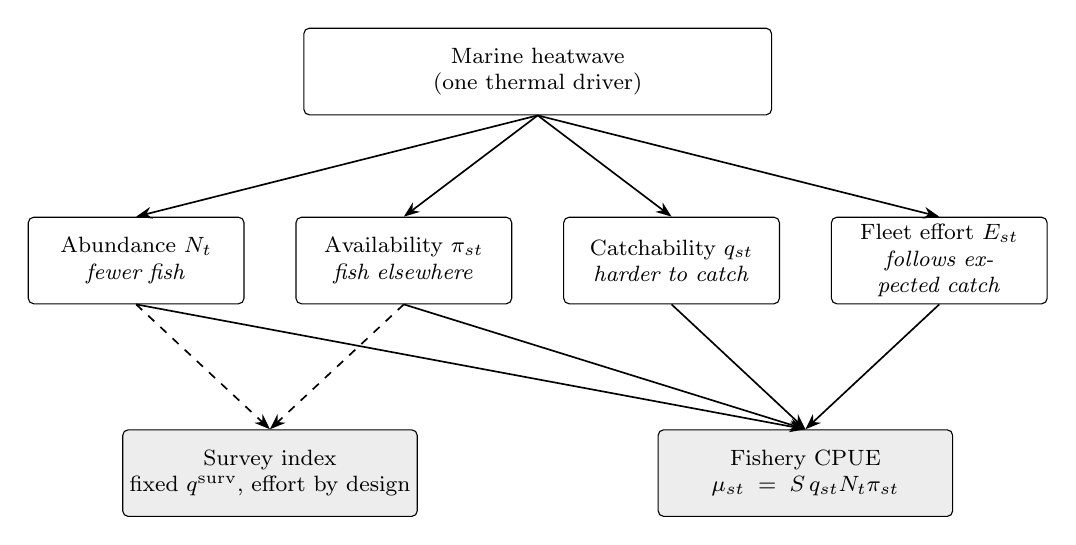
\begin{tikzpicture}[
  box/.style={draw, rounded corners=2pt, align=center, font=\footnotesize,
              text width=26mm, minimum height=11mm, inner sep=2pt},
  obs/.style={box, fill=black!7},
  arr/.style={-{Stealth[length=2mm]}, semithick}]
\node[box, text width=58mm] (mhw) at (51mm,24mm) {Marine heatwave\\(one thermal driver)};
\node[box] (N)  at (0mm,0mm)   {Abundance $N_t$\\\textit{fewer fish}};
\node[box] (pi) at (34mm,0mm)  {Availability $\pi_{st}$\\\textit{fish elsewhere}};
\node[box] (q)  at (68mm,0mm)  {Catchability $q_{st}$\\\textit{harder to catch}};
\node[box] (E)  at (102mm,0mm) {Fleet effort $E_{st}$\\\textit{follows expected catch}};
\node[obs, text width=36mm] (cpue) at (85mm,-27mm) {Fishery CPUE\\$\mu_{st}=S\,q_{st}N_t\pi_{st}$};
\node[obs, text width=36mm] (surv) at (17mm,-27mm) {Survey index\\fixed $q^{\text{surv}}$, effort by design};
\foreach \x in {N,pi,q,E} \draw[arr] (mhw.south) -- (\x.north);
\foreach \x in {N,pi,q,E} \draw[arr] (\x.south) -- (cpue.north);
\foreach \x in {N,pi} \draw[arr, dashed] (\x.south) -- (surv.north);
\end{tikzpicture}
\caption{Structure of the problem. One thermal driver acts on abundance, availability and catchability, and on where the fleet fishes. Fishery CPUE depends on all of them through a product, so a change in total abundance and a change in catchability that is the same everywhere leave identical fishery data. The survey (dashed inputs) has fixed catchability and effort set by design, so it receives no input from catchability or the fleet; this is why it can separate abundance from catchability inside the sampling frame, and why it cannot see fish that leave the frame.}
\label{fig:schematic}
\end{figure}

The invariance concerns only the part of catchability that is the same everywhere; a change confined to part of the range, such as the warm edge, cannot be absorbed by a single monthly factor $a_t$, so we treat it as a separate mechanism. Section~\ref{sec:res-ident} confirms the structural result numerically, and the experiments that follow show how large the practical problem is at realistic sample sizes.

\subsection{The mechanisms as an experimental design}
\label{sec:design}

The operating model lets each heatwave response be switched on or off. Three are mechanisms through which a heatwave changes catch rate: abundance decline, redistribution (a change in availability) and uniform catchability loss. The fourth is a response of the fleet: during an event it contracts onto the grid cells it knows best. Together they form a $2^4$ factorial of 16 scenarios, treated as a designed experiment so that main effects and interactions, including those between fleet contraction and the biological mechanisms, are estimated rather than assumed. Four further scenarios add a catchability loss confined to the warm edge of the range, with and without redistribution and fleet contraction, to test whether such a change can imitate real redistribution.

\subsection{What we estimate}
\label{sec:targets}

The quantity each index should recover is the effect of the heatwaves alone. To define it, every simulated data set is generated twice with the same random numbers: a run with the heatwaves, and a run with the heatwave anomaly removed while everything else (climatology, warming trend, noise, the fleet and its realised effort allocation) is held fixed. The difference between the two runs is the heatwave effect, and we use two versions of it as targets,
\begin{equation}
\Delta_t = \log N_t - \log N^0_t, \qquad \Delta^{\vt{in}}_t = \Delta_t + \log\big(1-\pi^{\vt{out}}_t\big) - \log\big(1-\pi^{\vt{out},0}_t\big),
\label{eq:targets}
\end{equation}
where the superscript $0$ marks the run without heatwaves. The effect on total abundance, $\Delta_t$, answers the question ``how many fish did the heatwaves remove from the stock?''. The effect on in-frame abundance, $\Delta^{\vt{in}}_t$, adds the change in the log proportion of the stock inside the frame and answers ``how many fewer fish are there in the area we can sample?''. Each series is reduced to a single number, its slope on centred heatwave severity $I_t$ (Section~\ref{sec:om}) after allowing for a linear trend and a seasonal cycle,
\begin{equation}
y_t = \alpha + \beta\, I_t + \zeta_1 \tfrac{t}{T} + \zeta_2 \sin\tfrac{2\pi t}{12} + \zeta_3 \cos\tfrac{2\pi t}{12} + \xi_t ,
\label{eq:regression}
\end{equation}
which gives the target $\beta$ when $y_t$ is the total-abundance series and $\beta^{\vt{in}}$ when it is the in-frame series. The same regression is applied to every estimated log index, so that every estimate and every target refers to the same quantity.

The two targets differ only when a heatwave moves fish across the edge of the frame, and a survey of the frame can be unbiased only for the second; which one a manager needs depends on whether the stock beyond the edge is still the stock being managed. Defining the targets by paired runs separates the heatwave effect from background warming and seasonality, although in our setting a simple regression of factual log abundance on severity gives almost the same value (within 0.002). Box~2 collects the key terms.

\begin{figure}[tb]
\centering
\fbox{\begin{minipage}{0.94\linewidth}
\small
\textbf{Box 2. Key terms}
\begin{description}\setlength{\itemsep}{1pt}
\item[Abundance] the population state: the number or biomass of fish in the whole stock.
\item[Availability] the proportion of the stock that is where the fleet fishes, and so could be caught.
\item[Catchability] the fraction of available fish taken by one unit of effort.
\item[Sampling frame] the area that the fishery and the survey can reach; in-frame abundance is the abundance inside it.
\item[Target (estimand)] the true quantity an index is meant to recover: here, the effect of the heatwaves alone on total or on in-frame abundance, defined by rerunning the same simulated fishery without the heatwave anomaly.
\item[Identifiable] two quantities are identifiable if different values of them produce different data; if not, no amount of data can separate them.
\item[Delta model] a two-part model of catch: whether any fish are caught, and how many when some are.
\item[Centre of gravity] the density-weighted mean poleward position of the stock, or the catch-rate-weighted mean position of fishery catches.
\item[Scenario, replicate] a scenario is one combination of mechanisms; a replicate is one simulated data set from it. Results are averages over replicates.
\end{description}
\end{minipage}}
\end{figure}

% =============================================================================
\section{Methods}

\subsection{Overview of the simulation}
\label{sec:overview}

Each replicate simulates eight years (96 months) of a fishery on a $12\times12$ grid of 50~km cells, with an open poleward edge and a refuge band beyond it (Figure~\ref{fig:schematic}). Month 1 is the initial state. In each later month the simulation runs in one sequence: the fleet allocates effort from its belief at the end of the previous month, abundance carries the removals implied by that effort, and catch is drawn from that abundance. The run without heatwaves (Section~\ref{sec:targets}) repeats the state process with the realised effort allocation and every random draw held fixed. Table~\ref{tab:settings} defines every symbol used below with its default value, and Table~\ref{tab:experiments} lists the experiments and the question each answers. Results are means over replicates. Scenarios share random numbers, so differences between scenarios are not inflated by simulation noise; the largest Monte Carlo standard error of any mean heatwave coefficient in the factorial is 0.0025.

\begin{table}[tbp]
\centering\footnotesize
\caption{Notation and default settings of the operating model, used in every experiment unless stated otherwise. Rates are per month; log abundance is relative to the carrying capacity; thermal stress is in degree-months.}
\label{tab:settings}
\begin{tabular}{@{}l>{\raggedright\arraybackslash}p{8.4cm}>{\raggedright\arraybackslash}p{3.4cm}@{}}
\toprule
Component & Symbol and meaning & Value \\
\midrule
Domain & grid of $S = n_{\vt{lat}}\times n_{\vt{shelf}}$ cells; cell size & $12\times12$; 50~km \\
 & series length $T$ & 96 months \\
Temperature & mean climatology $\bar{T}$ & 18.0\,$^\circ$C \\
 & cooling with latitude band $g_{\vt{lat}}$ and with cross-shelf band $g_{\vt{dep}}$ & 0.50 and 0.22\,$^\circ$C per band \\
 & seasonal amplitude $A$; phase $\varphi$ & 3.0\,$^\circ$C; 0.6 radians \\
 & warming trend $\omega$ & 0.05\,$^\circ$C per year \\
 & noise SD $\sigma_\varepsilon$; spatial kernel decay per cell $\rho_s$; temporal correlation $\rho_t$ & 0.40\,$^\circ$C; 0.55; 0.50 \\
Heatwaves & episodes per series $K$; duration & 6; 1 to 4 months \\
 & peak anomaly, mean (SD) & 2.2 (0.7)\,$^\circ$C \\
 & category one threshold $\tau$ & 1.0\,$^\circ$C \\
Thermal niche & optimum $T_{\vt{opt}}$; breadth $\sigma_{\vt{th}}$; stress threshold $T_{\vt{crit}}$ & 20.0; 1.9; 21.0\,$^\circ$C \\
Movement & adjustment rate $\rho_m$ (fraction of the gap to the target closed per month) & 0.55 \\
Abundance & recovery rate $r_0$; carrying capacity $K_{\vt{cap}}$; natural mortality $M$ & 0.09; 1.0; 0 \\
 & sensitivity to thermal stress $\kappa$; response lag $L$ & 0.12; 0 months \\
 & fishing mortality scale $f$; process noise SD $\sigma_{\vt{proc}}$ & $1.2\times10^{-4}$; 0.020 \\
Catchability & base $q_0$; uniform loss $\delta_{\vt{dep}}$; warm-edge loss $\delta_{\vt{sp}}$; concentration $\gamma_{\vt{sp}}$ & 1.0; 0.07; 0.16; 1.40 \\
Fishery catch & encounter scale $a_0$; lognormal SD $\sigma_{\log}$ & 0.9; 0.6 \\
Fleet & total effort $E_{\vt{tot}}$; vessels; vessel efficiency SD & 60 tows per month; 8; 0.25 \\
 & targeting strength $\beta_\mu$; contraction $\beta_J$; travel cost $\beta_{\vt{dist}}$ & 2.0; 0.8; 0.15 \\
 & learning rate $\psi$ (weight on the latest month's catch rate, dimensionless) & 0.5 \\
Survey & catchability $q^{\vt{surv}}$; encounter scale $a^{\vt{surv}}$; CV of positive tows & 1.0; 3.0; 0.45 \\
 & coverage $c$; frequency $k$; design & 0.10; monthly; simple random \\
\bottomrule
\end{tabular}
\end{table}

\begin{table}[tbp]
\centering\footnotesize
\caption{The experiments, the question each answers, and their size.}
\label{tab:experiments}
\begin{tabular}{@{}>{\raggedright\arraybackslash}p{0.16\linewidth}>{\raggedright\arraybackslash}p{0.35\linewidth}>{\raggedright\arraybackslash}p{0.32\linewidth}l@{}}
\toprule
Experiment & Question & Scenarios and replicates & Section \\
\midrule
Identifiability & Which heatwave responses can fishery data separate at all? & reduced likelihood on one simulated series & \ref{sec:res-ident} \\
Matched grid & Do different mixtures of decline and catchability loss give the same nominal coefficient? & $5\times5$ grid of decline rate $\kappa$ and catchability loss $\delta_{\vt{dep}}$ with fleet contraction, 80 replicates per point & \ref{sec:res-ident} \\
Factorial & Which index recovers which target under each combination of mechanisms? & 16 factorial and 4 warm-edge scenarios, 400 replicates each & \ref{sec:res-factorial}, \ref{sec:res-cog} \\
Survey design & How many stations, and how often, does a survey need? & 25 designs in the decline plus uniform catchability scenario with fleet contraction, 300 replicates each & \ref{sec:res-survey} \\
Frame geometry & Does the edge of the sampling frame change the answer? & 4 redistribution scenarios under 3 frame settings, 250 replicates each & \ref{sec:res-frame} \\
Temporal & Can a same-month model capture a lagged, cumulative decline? & one scenario with a 3-month lag, 300 replicates & \ref{sec:res-temporal} \\
Sensitivity & Which settings of the simulated fishery drive the results? & 15 parameters, 200 design points with 20 replicates each & \ref{sec:res-sens} \\
Diagnostic key & Can the joint pattern of the indices name the mechanism? & 5 factorial and 2 warm-edge scenarios with fleet contraction, split into training and test halves & \ref{sec:res-key} \\
\bottomrule
\end{tabular}
\end{table}

\subsection{Operating model}
\label{sec:om}

\subsubsection{Temperature and heatwaves}

Sea temperature in each grid cell and month is built from parts that can be removed one at a time, so that the run without heatwaves is well defined:
\begin{equation}
T_{st} = \underbrace{\bar{T} - g_{\vt{lat}}\,\ell_s - g_{\vt{dep}}\,c_s}_{\vt{climatology}} + \underbrace{A\sin\!\left(\tfrac{2\pi t}{12} - \varphi\right)}_{\vt{season}} + \underbrace{\omega\,\tfrac{t}{12}}_{\vt{trend}} + \underbrace{\varepsilon_{st}}_{\vt{noise}} + \underbrace{H_{st}}_{\vt{heatwave}} ,
\label{eq:temp}
\end{equation}
where $\ell_s$ and $c_s$ are the latitude band and cross-shelf band of cell $s$, $\bar T$ the mean climatology, $g_{\vt{lat}}$ and $g_{\vt{dep}}$ the cooling per band poleward and offshore, $A$ and $\varphi$ the seasonal amplitude and phase, and $\omega$ the warming trend (Table~\ref{tab:settings}). The noise $\varepsilon_{st}$ has standard deviation $\sigma_\varepsilon$; it is smoothed in space by a kernel whose weight falls by a factor $\rho_s$ for each cell of distance, which makes neighbouring cells strongly correlated, and it is autocorrelated between consecutive months ($\rho_t$). The heatwave anomaly $H_{st}\ge0$ is zero outside events and is deleted in the run without heatwaves, whose temperature we write $T^0_{st}$.

Heatwaves follow a schedule of $K$ episodes per series, with random start months, durations of one to four months and peak anomalies near 2.2\,$^\circ$C; overlapping episodes merge. Within an episode the anomaly rises and decays smoothly. Its strength in each month is summarised by a severity index, the intensity above the category one threshold $\tau$ in units of that threshold,
\begin{equation}
J_t = \frac{\max(H_t - \tau,\ 0)}{\tau}, \qquad H_t = \frac{1}{S}\sum_s H_{st},
\label{eq:severity}
\end{equation}
which is zero in months without a heatwave and grows with its intensity. Catchability and the fleet respond to $\hat J_t$, the severity scaled to unit standard deviation over event months (and zero in a run without events); abundance and distribution respond to temperature itself, through the thermal niche, so an anomaly below the category one threshold still stresses the stock although it does not register in $J_t$. The estimators receive a different covariate, the centred and scaled severity $I_t = (J_t - \bar J)/\mathrm{sd}(J)$, so that no estimator is handed the sign of the true response through its covariate.

\subsubsection{Thermal suitability and movement}

Habitat suitability is a Gaussian function of the distance between local temperature and the thermal optimum $T_{\vt{opt}}$,
\begin{equation}
h_{st} = \exp\!\left(-\frac{(T_{st}-T_{\vt{opt}})^2}{2\,\sigma_{\vt{th}}^2}\right),
\label{eq:suit}
\end{equation}
where $\sigma_{\vt{th}}$, the niche breadth, sets how fast suitability falls away from the optimum. The sampling frame is open at its poleward edge. One latitude band beyond it lies a refuge whose temperature follows the same climatological gradient, season, trend and heatwave anomaly as the frame, $T^{\vt{ref}}_t = \bar T - g_{\vt{lat}}(n_{\vt{lat}}+1-\bar\ell) + A\sin(2\pi t/12-\varphi) + \omega t/12 + H_t$, with suitability $h^{\vt{ref}}_t$ from the same niche and the area of one band, $w^{\vt{ref}} = n_{\vt{shelf}}$. When redistribution is switched on, the stock moves part of the way each month toward the distribution that suitability alone would imply, the ideal free distribution \citep{fretwell1969},
\begin{equation}
\pi_{st} = (1-\rho_m)\,\pi_{s,t-1} + \rho_m\,\tilde h_{st}, \qquad \pi^{\vt{out}}_t = (1-\rho_m)\,\pi^{\vt{out}}_{t-1} + \rho_m\,\tilde h^{\vt{ref}}_t,
\label{eq:move}
\end{equation}
with $\tilde h_{st} = h_{st}\big/\big(\sum_{s'}h_{s't} + w^{\vt{ref}}h^{\vt{ref}}_t\big)$, $\tilde h^{\vt{ref}}_t$ defined likewise, and the proportions renormalised each month. The adjustment rate $\rho_m$ controls how quickly fish follow the suitability surface. Fish therefore leave the frame only when conditions beyond its edge are better than within it, which here happens in warm seasons and during events. When redistribution is switched off, the proportions are fixed at the mean suitability over the series without heatwaves, the same in both runs, so that no heatwave enters the paired contrast through the distribution. A refuge whose suitability is fixed in time is used as a comparison in Section~\ref{sec:res-frame}: it responds neither to the season nor to events, so biomass leaves the frame toward it in normal conditions and returns when a heatwave warms the frame toward the thermal optimum.

\subsubsection{Abundance}

Abundance changes on the log scale through density-dependent recovery, natural and fishing mortality, and, when the decline mechanism is on, a response to the thermal stress the stock experienced $L$ months earlier:
\begin{equation}
\log N_t = \log N_{t-1} + r_0\!\left(1-\frac{N_{t-1}}{K_{\vt{cap}}}\right) - M - F_t - \kappa\,d_{t-L} + \eta_t, \qquad \eta_t\sim\mathcal{N}(0,\sigma^2_{\vt{proc}}),
\label{eq:abund}
\end{equation}
for $t = 2,\dots,T$, with $N_1$ the initial state. Here $r_0$ is the intrinsic recovery rate, $K_{\vt{cap}}$ the carrying capacity, $M$ natural mortality and $\kappa$ the sensitivity of abundance to thermal stress. Fishing mortality is proportional to the expected catch per unit abundance implied by that month's effort,
\begin{equation}
F_t = f\,S\sum_{s=1}^{S} q_{st}\,\pi_{st}\,E_{st} \;\ge 0,
\label{eq:F}
\end{equation}
so it rises with the overlap between fleet and stock and falls when catchability falls. Thermal stress is accumulated over the frame, weighted by where the stock is,
\begin{equation}
d_t = \sum_{s=1}^{S}\pi_{st}\,\max(T_{st}-T_{\vt{crit}},\ 0),
\label{eq:dose}
\end{equation}
with $T_{\vt{crit}}$ a stress threshold above the thermal optimum. Fish beyond the frame edge are neither fished nor stressed; the refuge is cooler than the frame and exceeds $T_{\vt{crit}}$ in fewer than 0.1 percent of months, so the omitted stress is negligible (Supporting Information, Section~S2).

\subsubsection{Catchability}

Catchability has two parts: one that is the same everywhere, which is the part confounded with abundance, and one concentrated at the warm edge of the range,
\begin{equation}
q_{st} = q_0 \cdot \underbrace{\exp\!\left(-\delta_{\vt{dep}}\,\hat J_t\right)}_{\vt{uniform}} \cdot \underbrace{\exp\!\left(-\delta_{\vt{sp}}\,g_s\,\hat J_t\right)}_{\vt{warm edge}},
\label{eq:q}
\end{equation}
where $g_s = v_s/\bar v$ and $v_s = \max(1-\gamma_{\vt{sp}}\,y_s,\ 0)$, with $y_s$ the standardised poleward coordinate of the cell. The weight $g_s$ is largest at the warm, equatorward edge and averages one over the frame, so the second term concentrates the loss where water is warmest. The two parts can be used separately or together.

\subsection{How the fishery and the survey observe the stock}

\subsubsection{Fishery catch}

A grid cell that receives $E_{st}$ tows of effort records at least one encounter, a tow with positive catch, with probability
\begin{equation}
p_{st} = 1-\exp(-a_0\,\mu_{st}\,E_{st}),
\label{eq:encounter}
\end{equation}
and, given an encounter, its catch rate (the mean over its tows) is lognormal with a variance that falls as effort rises,
\begin{equation}
Y_{st}\mid\vt{encounter} \sim \vt{Lognormal}\!\left(\log\frac{\mu_{st}}{p_{st}} - \frac{\sigma^2_{\log}}{2E_{st}},\ \frac{\sigma^2_{\log}}{E_{st}}\right), \qquad \Pr(Y_{st}=0) = 1-p_{st}.
\label{eq:catch}
\end{equation}
The two parts are matched so that the expected catch rate equals $\mu_{st}$ at any level of effort, $\mathbb{E}[Y_{st}] = p_{st}\cdot\mu_{st}/p_{st} = \mu_{st}$, and the zero catches that dominate real records enter every index that keeps them. Catch is drawn from the abundance of the same month after that month's removals, so observations and truth always refer to one state. There is no gear saturation or depredation in the model.

\subsubsection{Fleet behaviour}

Total monthly effort $E_{\vt{tot}}$ is shared among grid cells by a multinomial draw based on the fleet's belief at the end of the previous month and on the current month's heatwave severity,
\begin{equation}
(E_{1t},\dots,E_{St}) \sim \vt{Multinomial}\big(E_{\vt{tot}},\ w_{1t},\dots,w_{St}\big), \qquad w_{st} = \frac{\exp(u_{st})}{\sum_{s'}\exp(u_{s't})},
\label{eq:effort}
\end{equation}
where the attractiveness $u_{st}$ of a cell combines the fleet's belief about its catch rate, the cost of travel from port (with $\vt{dist}_s$ the scaled distance of the cell from port) and a vessel efficiency effect $\nu_{v(s)}$,
\begin{equation}
u_{st} = \beta_\mu\big(1+\beta_J\,\hat J_t\,\mathbf{1}\{\vt{contraction}\}\big)\,b_{s,t-1} - \beta_{\vt{dist}}\,\vt{dist}_s + \nu_{v(s)} .
\label{eq:score}
\end{equation}
Here $\beta_\mu$ is the strength of targeting and $\mathbf{1}\{\cdot\}$ equals one when fleet contraction is switched on. During an event the contraction term sharpens targeting, so effort concentrates on fewer, better-known cells and the fished footprint shrinks. Contraction has to enter as an interaction with targeting strength: a term added equally to every cell's score would cancel in the softmax of eq.~\eqref{eq:effort} and leave the allocation unchanged. The belief is a running blend of past and current experience,
\begin{equation}
b_{st} = (1-\psi)\,b_{s,t-1} + \psi\,z_{st},
\label{eq:belief}
\end{equation}
where $z_{st}$ is the log catch rate observed in cell $s$ in month $t$, standardised across cells, with the previous belief carried forward for cells left unfished, and $\psi$ is the weight placed on the latest month. Effort is generated rather than assumed, so CPUE is catch divided by effort throughout, as in a real fishery.

\subsubsection{Survey}

The fishery-independent survey visits $n=\max\{1,\operatorname{round}(cS)\}$ grid cells, drawn without replacement, once every $k$ months ($k=1$ monthly, 3 quarterly, 6 twice-yearly), by simple random sampling or with equal allocation across latitude bands. Stratification needs at least one station per band, so designs with fewer stations than bands revert to simple random sampling. Both designs give every cell the same inclusion probability, $p^{\vt{inc}} = n/S$, so stratification changes the variance of the estimator but not its form. Survey catches follow their own delta-lognormal model, with catchability $q^{\vt{surv}}$ and encounter scale $a^{\vt{surv}}$ fixed by protocol; neither responds to the heatwave. Its index is a Horvitz--Thompson estimate of the total, and its centre of gravity a Hájek ratio \citep{horvitz1952,sarndal1992},
\begin{equation}
\widehat B_t = \sum_{s\in\mathcal S_t}\frac{V_{st}}{p^{\vt{inc}}}, \qquad \widehat G_t = \frac{\sum_{s\in\mathcal S_t} y_s\,V_{st}}{\sum_{s\in\mathcal S_t}V_{st}},
\label{eq:survey}
\end{equation}
where $\mathcal S_t$ is the set of cells sampled in month $t$ and $V_{st}$ the survey catch. The total estimates $S\,q^{\vt{surv}}N_t(1-\pi^{\vt{out}}_t)$, the abundance inside the frame, not total abundance. In a month in which no station catches anything the total is zero and its logarithm undefined; such months are set to half the smallest positive total in the series, and their number is reported.

A survey also divides catch by effort; what differs is that its stations are drawn with known inclusion probabilities that do not depend on abundance, its gear and protocol are fixed so that $q^{\vt{surv}}$ does not carry the factor that eq.~\eqref{eq:invariance} confounds with abundance, and it samples the whole frame, including the warm edge the fleet abandons. These are design choices, and a survey that violated them would be as confounded as the fishery (Supporting Information, Section~S1).

\subsection{Estimators and how they are compared}
\label{sec:estimators}

We compare a graded sequence of estimators, so that errors removable through better modelling are separated from limitations intrinsic to the data. Each produces a monthly log index $y_t$.

\paragraph{Nominal index.} Total catch over total effort,
\begin{equation}
y^{\vt{nom}}_t = \log\frac{\sum_s Y_{st}E_{st}}{\sum_s E_{st}\,\mathbf{1}\{Y_{st}\ \vt{observed}\}},
\label{eq:nominal}
\end{equation}
the simplest index and the baseline for the others.

\paragraph{Positive-only index.} The mean log catch rate of positive catches after removing grid-cell and calendar-month means. It discards zero catches and stands in for a practice that delta models are meant to replace.

\paragraph{Delta index.} Two models with additive grid-cell and month effects, one for encounters and one for positive catches,
\begin{equation}
\operatorname{logit} p_{st} = a^{\vt{enc}}_s + m^{\vt{enc}}_t, \qquad \log Y_{st}\mid(Y_{st}>0) = \beta^{\vt{pos}}_0 + a^{\vt{pos}}_s + m^{\vt{pos}}_t + e_{st},
\label{eq:delta}
\end{equation}
with a light ridge penalty on the encounter effects of grid cells, since a cell in which fish are never encountered has no finite maximum-likelihood estimate. The index is the prediction over the complete grid,
\begin{equation}
y^{\delta}_t = \log\left(\frac1S\sum_{s=1}^S \hat p_{st}\,\exp\!\big(\hat\beta^{\vt{pos}}_0 + \hat a^{\vt{pos}}_s + \hat m^{\vt{pos}}_t + \tfrac12\hat\sigma^2\big)\right),
\label{eq:deltaindex}
\end{equation}
so that it reflects modelled density rather than where effort happened to go. Effort per cell is not a covariate: total effort is fixed, and fleet contraction changes effort per fished cell by about 8 percent during events, which an effort-adjusted version of the index shows to be immaterial (Supporting Information, Section~S3). The fleet leaves most grid cells unfished in any month, and the prediction for those cells is an imputation; we report its share, together with a variant that averages only over the cells fished in each month.

\paragraph{Spatial delta index.} The delta index with a low-dimensional interaction between position and severity, $\mathbf{z}_s^{\top}\boldsymbol{\theta}\,I_t$ with $\mathbf{z}_s = (y_s, x_s)$ the poleward and offshore coordinates, added to each component. Its density surface can move with the event, which a purely additive model cannot do, so it also yields a centre of gravity \citep{thorson2016a}.

\paragraph{Survey index.} The design-based total of eq.~\eqref{eq:survey}.

Every index is reduced to a heatwave coefficient by the regression of eq.~\eqref{eq:regression}, the same regression that defines the targets. Standard errors use the Newey--West estimator with a Bartlett kernel and three lags \citep{newey1987}, which allows for autocorrelation in the monthly residuals and lets us report, for each estimator, the coverage of its 95 percent interval and its power to reject a zero effect. Accuracy is summarised by bias, root mean squared error (RMSE) and median absolute error against each target. A heatwave coefficient is the change in the log index for a one standard deviation increase in severity. At the sizes reported here it is close to a proportional change: a coefficient of $-0.023$ corresponds to a decline of about 2.3 percent per standard deviation of severity, and $-0.064$ to about 6 percent.

\subsection{Spatial and temporal diagnostics}
\label{sec:diagnostics}

\paragraph{Centre of gravity.} Three measures of where the stock is are compared with the true centre of gravity, $G_t = \sum_s y_s\,\pi_{st}\big/\sum_s\pi_{st}$. The fishery's centre of gravity weights the cells with positive catch by their catch rate,
\begin{equation}
G^{\vt{fish}}_t = \frac{\sum_{s\in\mathcal{P}_t} y_s\,Y_{st}}{\sum_{s\in\mathcal{P}_t} Y_{st}},
\label{eq:cog}
\end{equation}
where $\mathcal{P}_t$ is the set of fished cells with positive catch in month $t$. It describes where catch rates were high among the cells the fleet chose to fish; it indicates fishery use and is not an unbiased estimator of the stock's location. The centre of gravity of the spatial delta index surface estimates the stock's distribution, and the survey's is the Hájek ratio of eq.~\eqref{eq:survey}. Each is summarised by its event contrast, the mean poleward position during event months minus the mean outside them. Shifts are reported in kilometres: one unit of the standardised coordinate $y_s$ spans 3.46 latitude bands, or 173~km.

\paragraph{Lagged responses.} The temporal experiment gives abundance a three-month lag with slower recovery and greater sensitivity ($L=3$, $r_0=0.05$, $\kappa=0.16$, $\sigma_{\vt{proc}}=0.010$), with decline and fleet contraction active and a monthly survey covering 20 percent of the grid. A same-month model, $y_t = \alpha + \beta I_t + \xi_t$, is compared with a penalised distributed lag over the previous 24 months whose smoothing is chosen by generalised cross-validation \citep[Supporting Information, Section~S4;][]{craven1979}. Both are fitted to the detrended survey index, which an analyst can observe, and to the true heatwave effect, which bounds what any lag model could recover, and compared in sample and on blocked out-of-sample prediction with the smoothing re-selected inside each training block.

\paragraph{Global sensitivity.} Fifteen parameters are varied together over a Latin hypercube of 200 design points within the ranges of Table~S1, each simulated with 20 replicates of the scenario with all four mechanisms active. Outcomes are summarised by standardised regression coefficients: the change in the outcome, in standard deviations, for a one standard deviation change in one parameter with the others held fixed.

\paragraph{A diagnostic key.} The heatwave coefficients of the delta and survey indices and the event contrasts of the fishery and survey centres of gravity are each flagged when they exceed a threshold learned from no-effect replicates, and the pattern of flags names a mechanism (Supporting Information, Section~S5). The key is learned on half of the replicates of seven scenarios with fleet contraction and tested on the other half.

\subsection{Computation}

All simulations, estimators, tables and figures are implemented in R (Data availability). Replicate seeds are a deterministic function of the replicate index, so scenarios share random numbers and results are reproducible. A test suite checks, among other properties, that fishing mortality is never negative, that the survey is unbiased for in-frame abundance, and that the paired contrast is exactly zero before the first heatwave anomaly when redistribution is off.

% =============================================================================
\section{Results}

The operating model behaves as intended (Figure~\ref{fig:fields}). During a heatwave the domain warms, the stock contracts toward the cool poleward edge, and catchability falls at the warm edge, all emerging from the single thermal driver. The simulated data have the features that make real CPUE hard to interpret: a strongly seasonal temperature series punctuated by events, catch rates that are zero in 36 to 55 percent of fished cells (43 percent on average across scenarios) and right-skewed where positive, and a fished footprint that fluctuates with the fleet's beliefs (Figure~S1). Figure~\ref{fig:traj} makes the confounding concrete: under each mechanism the observed indices are plotted against both targets over time, and the nominal index departs from them event by event.

\begin{figure}[tbp]
\centering
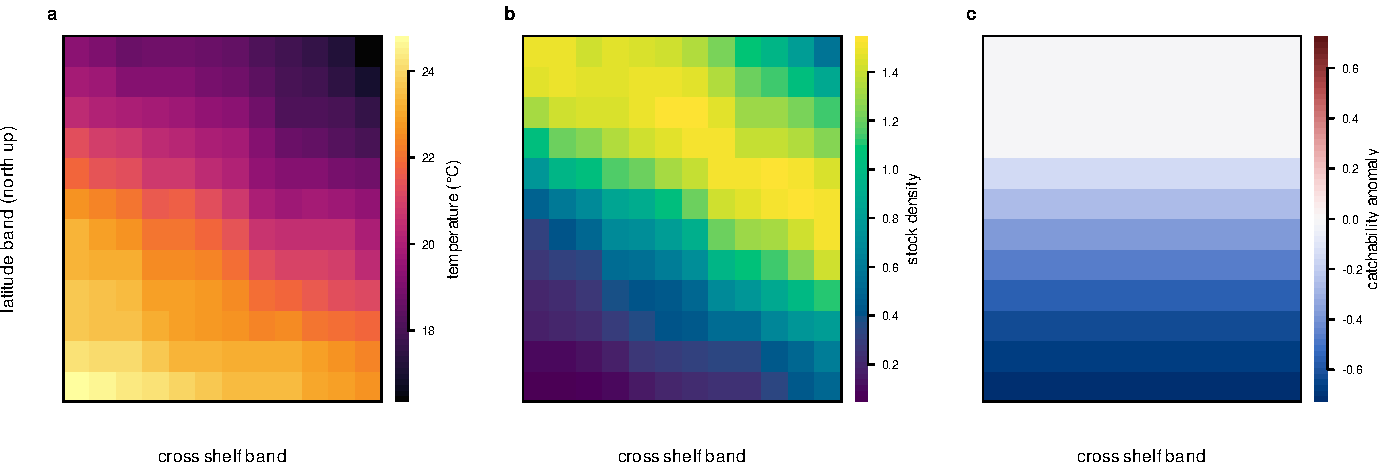
\includegraphics[width=\linewidth]{fig1_spatial_fields.pdf}
\caption{Spatial fields at the peak of a heatwave in a replicate with every mechanism active, including warm-edge catchability loss. (a) Sea temperature over the grid (north up, inshore at left). (b) Stock density, contracted toward the cool poleward edge. (c) Catchability relative to its pre-event level, reduced at the warm equatorward edge.}
\label{fig:fields}
\end{figure}

\begin{figure}[tbp]
\centering
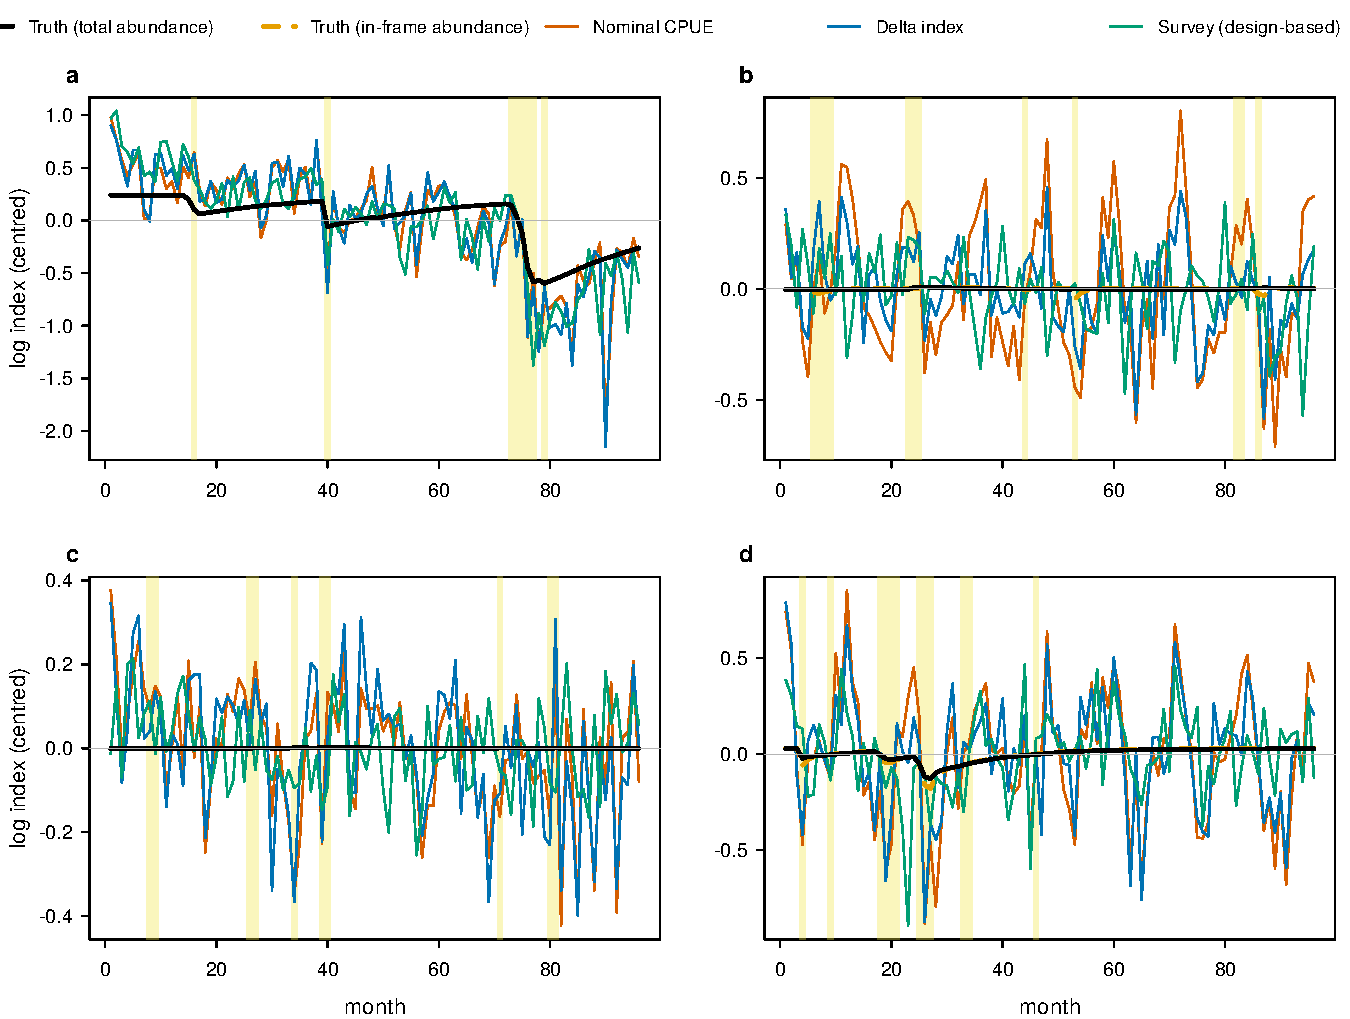
\includegraphics[width=\linewidth]{fig3_trajectories.pdf}
\caption{Index trajectories in one representative replicate of four scenarios, all with fleet contraction active: (a) abundance decline, (b) redistribution, (c) uniform catchability loss, (d) all three. Heatwave months are shaded. The heatwave effect on total abundance (black) and on in-frame abundance (orange dashed) are shown with the nominal, delta and survey indices, all centred. Under redistribution the two targets separate and the survey follows the in-frame target. Colours identify estimators consistently across all figures.}
\label{fig:traj}
\end{figure}

\subsection{Fishery data cannot split abundance from uniform catchability}
\label{sec:res-ident}

A decline in CPUE can reflect fewer fish or fish that are uniformly harder to catch, and fishery data alone cannot distinguish the two. The likelihood geometry makes this explicit (Figure~\ref{fig:ident}a). In a reduced likelihood with one slope for abundance decline and one for uniform catchability loss, the fishery-only information matrix has eigenvalues of about 1209 and 0, the second zero to numerical precision, and the profile likelihood for the abundance slope changes by less than $2\times10^{-7}$ log-likelihood units across a range of 0.9 in the slope. Adding survey observations with fixed catchability breaks this confounding: the eigenvalues become about 2287 and 387, and the profile likelihood falls by 322 log-likelihood units over the same range.

A catchability change confined to the warm edge behaves differently. Because it varies across space, it leaves a detectable signature. Adding a warm-edge catchability slope gives a three-parameter fishery information matrix with eigenvalues of about 2900, 186 and $5\times10^{-13}$. The only remaining flat direction is the uniform abundance--catchability combination, and the profile likelihood for the warm-edge effect is curved from fishery data alone (Figure~\ref{fig:ident}b). With survey data added, all three eigenvalues are positive (3331, 1109 and 107).

The same pattern appears in the full simulation. Across a grid of decline rates and uniform catchability losses, distinct mechanisms produce nearly indistinguishable fishery signals (Figure~\ref{fig:ident}c,d). Catchability loss without decline ($\kappa=0$, $\delta_{\vt{dep}}=0.07$; true effect 0.000), a mixture of the two ($\kappa=0.06$, $\delta_{\vt{dep}}=0.035$; $-$0.013) and decline without catchability loss ($\kappa=0.12$, $\delta_{\vt{dep}}=0$; $-$0.024) yield nominal coefficients of $-$0.039, $-$0.038 and $-$0.032. The corresponding survey coefficients are $-$0.002, $-$0.017 and $-$0.024, correctly separating the scenarios. Fishery data can identify spatially structured catchability; they cannot identify spatially uniform catchability. That distinction organises the remainder of the results.

\begin{figure}[tbp]
\centering
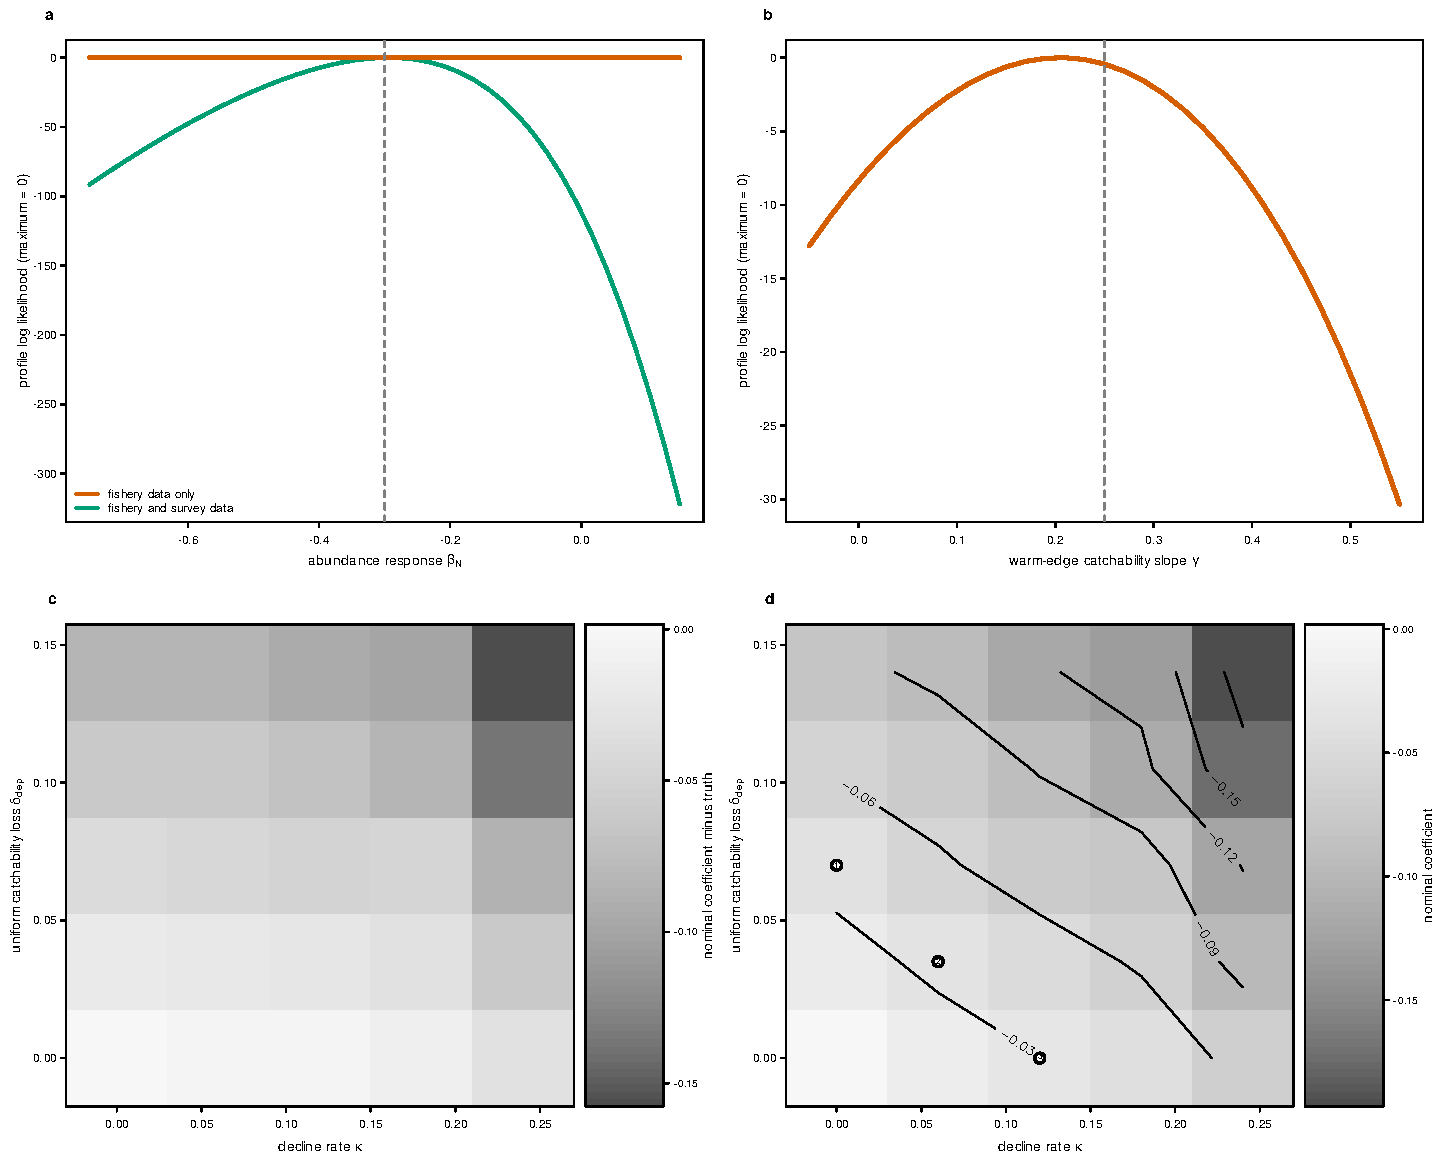
\includegraphics[width=\linewidth]{fig11_identifiability.pdf}
\caption{Fishery data cannot separate abundance from uniform catchability, but can detect a warm-edge catchability change. (a) Profile log likelihood of the abundance response $\beta_N$ from fishery data only (flat) and from fishery and survey data (curved); the dashed line marks the true value. (b) Profile log likelihood of the warm-edge catchability slope $\gamma$ from fishery data only, which is curved. (c) The nominal coefficient minus the true effect across a grid of decline rate $\kappa$ and uniform catchability loss $\delta_{\vt{dep}}$, with fleet contraction active (80 replicates per grid point); darker cells are further from the truth. (d) The nominal coefficient over the same grid. Contours join combinations that give the same observed coefficient; the numbered points mark the three cases compared in the text (1, catchability loss only; 2, both; 3, decline only).}
\label{fig:ident}
\end{figure}

\subsection{Which indices recover which target}
\label{sec:res-factorial}

Figure~\ref{fig:effects} and Table~\ref{tab:coef} report heatwave coefficients for all estimators with fleet contraction active, against both abundance targets; Table~S2 adds the scenarios without contraction, Table~S9 the factorial main effects and interactions, and Figure~S2 shows the sampling distributions. Three patterns dominate.

\paragraph{Abundance decline alone is recovered accurately.} When abundance declines without redistribution or catchability change, every estimator except the positive-only index recovers the true effect ($-$0.024): the nominal, delta, spatial delta and survey coefficients are all within 0.005 of the target, and without fleet contraction the nominal index is within 0.001 (Table~S2). The positive-only index is unstable because the zero catches it discards contain information about changes in availability and effort allocation.

\paragraph{Uniform catchability loss confounds every fishery index.} When catchability falls everywhere and abundance does not change, all fishery indices report substantial declines ($-$0.038 to $-$0.043) despite a true abundance effect of zero, while the survey remains centred on zero ($-$0.001). When abundance decline and catchability loss coincide, the fishery indices exaggerate the decline by almost a factor of three (nominal $-$0.069 against a true $-$0.023), while the survey reads $-$0.026. This is the structural confounding of Section~\ref{sec:res-ident} appearing in finite samples.

\paragraph{Redistribution separates total and in-frame abundance.} Redistribution moves fish beyond the poleward boundary, creating a divergence between total and in-frame abundance (0 against $-$0.010 under redistribution alone). The survey tracks the in-frame target ($-$0.008); across all ten redistribution scenarios its error against in-frame abundance is at most 0.004, comparable to the Monte Carlo standard error, while its error against total abundance is close to the proportion that left. The spatial delta index removes most redistribution bias when catchability is unchanged ($-$0.004 against $-$0.010, and $-$0.025 against $-$0.025 when decline and redistribution coincide), far closer than the nominal ($-$0.045) and fixed-shape delta ($-$0.035) indices. That advantage disappears once catchability also changes ($-$0.045 against $-$0.010). Redistribution therefore has a partial fishery-only remedy, available only when catchability remains constant, whereas uniform catchability loss has none.

\paragraph{Fleet contraction contributes little.} Contraction alone has a negligible effect (nominal coefficient 0.001 against a true effect of zero), and its interactions with the biological mechanisms are of order 0.003 (Table~S3). The full-grid and fished-cells delta indices differ by at most 0.004 in any scenario, so imputation of the roughly 70 percent of unfished cells does not drive the delta model's behaviour, and the delta index converged in every replicate.

\begin{figure}[tbp]
\centering
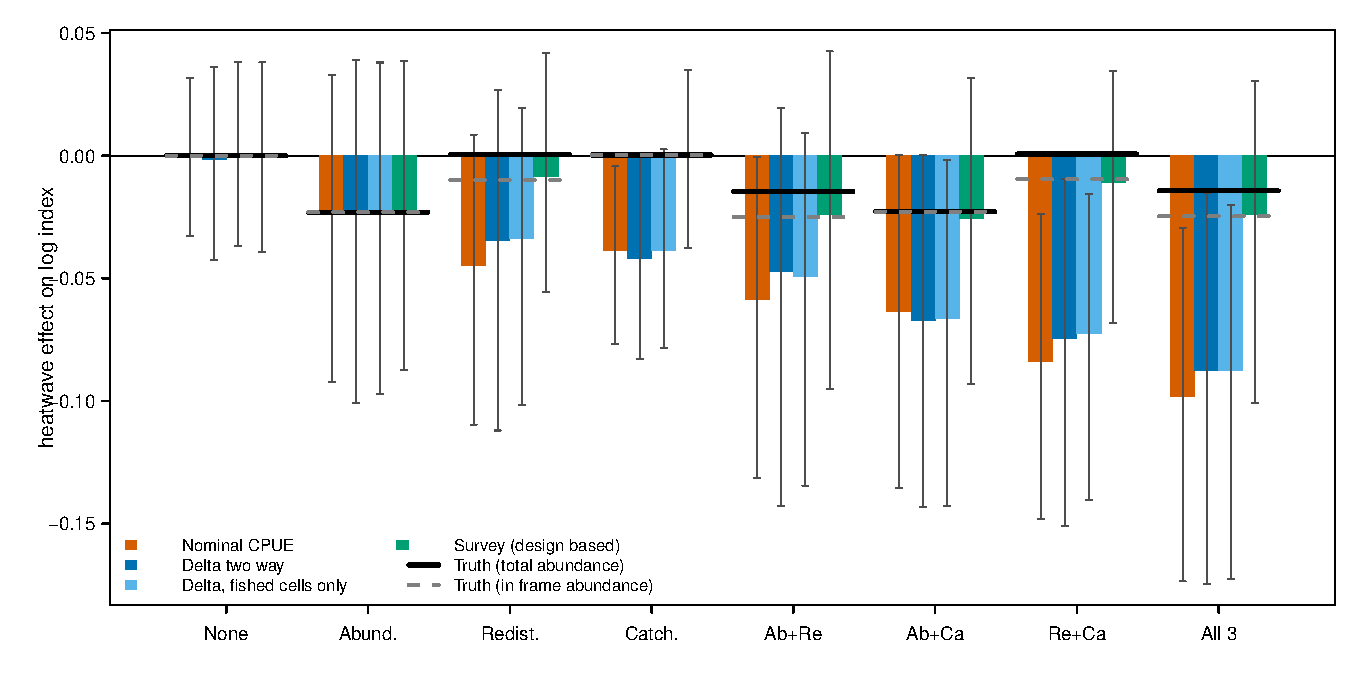
\includegraphics[width=\linewidth]{fig5_effect_by_case.pdf}
\caption{Heatwave coefficients for the ten scenarios with fleet contraction active: the eight combinations of abundance decline (Ab), redistribution (Re) and uniform catchability loss (Ca), and warm-edge catchability loss without (WE) and with redistribution (WE+Re). Bars give the mean coefficient of each estimator over 400 replicates and whiskers the central 95 percent of replicates; the black line is the effect on total abundance and the orange dashed line the effect on in-frame abundance. A bar that reaches the orange line is unbiased for in-frame abundance. The survey lands on the in-frame target in every scenario; no fishery index is robust to uniform catchability loss.}
\label{fig:effects}
\end{figure}

\begin{table}[tbp]
\centering\footnotesize
\setlength{\tabcolsep}{3.5pt}
\caption{Mean heatwave coefficient of each estimator by scenario, with fleet contraction active (400 replicates per scenario; largest Monte Carlo standard error 0.0025). The two target columns are the heatwave effects on total and on in-frame abundance; they differ only where redistribution moves fish across the frame edge. Table~S2 adds the scenarios without fleet contraction.}
\label{tab:coef}
\begin{tabular}{@{}>{\raggedright\arraybackslash}p{3.2cm}rrrrrrrr@{}}
\toprule
 & \multicolumn{2}{c}{Target} & \multicolumn{6}{c}{Estimator} \\
\cmidrule(lr){2-3}\cmidrule(l){4-9}
 & & & & Positive- & & Delta, & Spatial & \\
Scenario & Total & In-frame & Nominal & only & Delta & fished & delta & Survey \\
\midrule
None & 0.000 & 0.000 & 0.001 & $-$0.008 & 0.000 & 0.001 & $-$0.001 & 0.000 \\
Abundance decline & $-$0.024 & $-$0.024 & $-$0.028 & $-$0.028 & $-$0.028 & $-$0.029 & $-$0.028 & $-$0.024 \\
Redistribution & 0.000 & $-$0.010 & $-$0.045 & $-$0.029 & $-$0.035 & $-$0.034 & $-$0.004 & $-$0.008 \\
Uniform catchability loss & 0.000 & 0.000 & $-$0.038 & $-$0.027 & $-$0.043 & $-$0.039 & $-$0.042 & $-$0.001 \\
Decline + redistribution & $-$0.015 & $-$0.025 & $-$0.059 & $-$0.035 & $-$0.047 & $-$0.049 & $-$0.025 & $-$0.024 \\
Decline + catchability loss & $-$0.023 & $-$0.023 & $-$0.069 & $-$0.041 & $-$0.072 & $-$0.072 & $-$0.070 & $-$0.026 \\
Redistribution + catchability loss & 0.001 & $-$0.010 & $-$0.084 & $-$0.047 & $-$0.074 & $-$0.072 & $-$0.045 & $-$0.011 \\
All three & $-$0.014 & $-$0.025 & $-$0.098 & $-$0.049 & $-$0.088 & $-$0.088 & $-$0.063 & $-$0.024 \\
Warm-edge catchability loss & 0.001 & 0.001 & $-$0.107 & $-$0.054 & $-$0.110 & $-$0.105 & $-$0.095 & 0.000 \\
Warm-edge loss + redistribution & 0.001 & $-$0.009 & $-$0.141 & $-$0.063 & $-$0.129 & $-$0.126 & $-$0.078 & $-$0.009 \\
\bottomrule
\end{tabular}
\end{table}

\subsection{Only the survey separates movement from a warm-edge catchability artefact}
\label{sec:res-cog}

The centre of gravity separates real movement from a catchability artefact, but only when it is computed from the survey (Figure~\ref{fig:warmedge}, Table~\ref{tab:cog}). Under pure redistribution the stock's centre of gravity moves poleward by about 53~km during events. The fishery's centre of gravity moves by 45~km, the survey's by 49~km and that of the spatial delta index by 38~km, whereas the heatwave coefficient cannot register this movement at all, since the target on total abundance is zero. The warm-edge scenarios show why the fishery measure is not enough on its own. When catchability falls only at the warm edge, with no change in abundance or distribution, the fishery centre of gravity still moves poleward by 34~km, because catch rates fall in the warm-edge cells and the catch-rate-weighted mean moves away from them. The spatial delta surface shifts by about 32~km for the same reason, while the survey centre of gravity does not move (0.7~km). In the same scenario the nominal index reads $-$0.107 against a true effect of 0.001, a spurious decline of about 10 percent per standard deviation of severity. Combined with real redistribution, the warm-edge loss exaggerates the fishery's shift (71~km against a true 53~km), while the survey stays close to the truth (49~km). Only the survey tells the two explanations apart.

\begin{figure}[tbp]
\centering
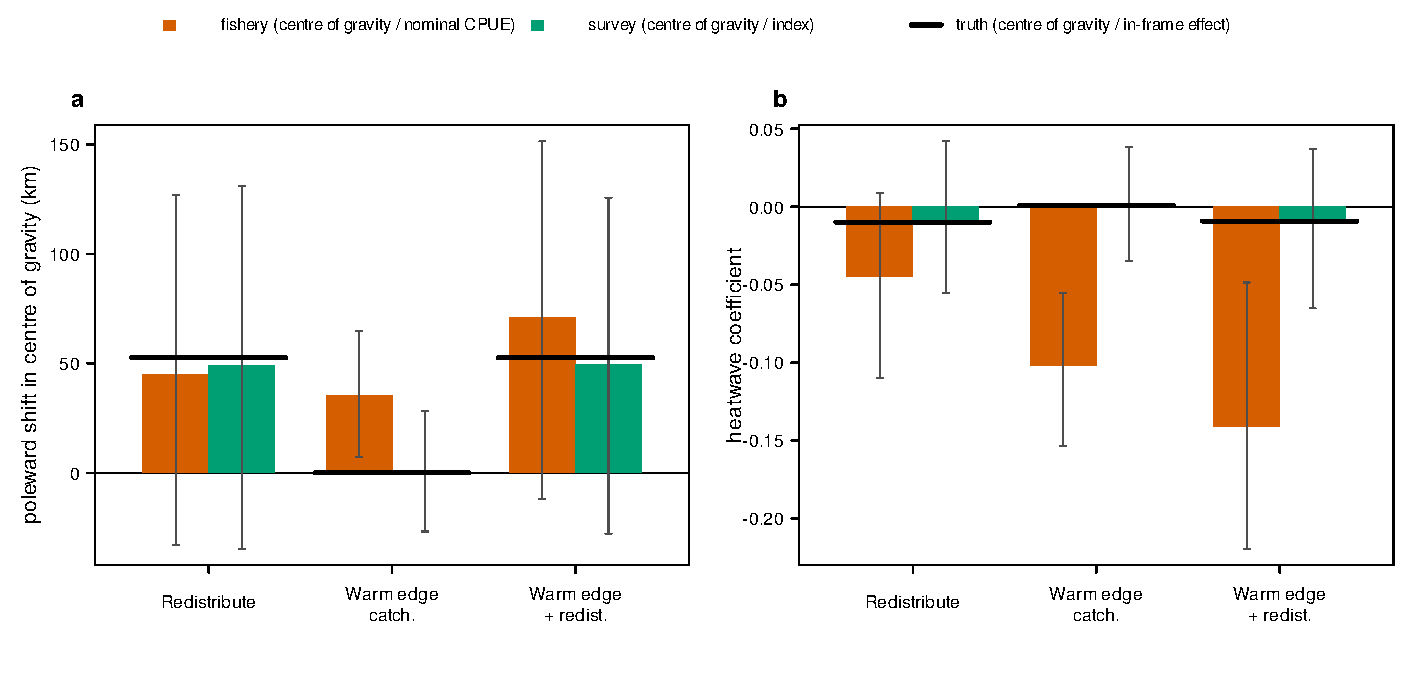
\includegraphics[width=\linewidth]{fig8_spatial_catchability.pdf}
\caption{Warm-edge catchability stress test, with fleet contraction active. (a) Poleward shift in the centre of gravity during events (km) for the fishery catch rates and for the survey, under redistribution, warm-edge catchability loss, and both; the black bar is the true shift of the stock. A bar above zero means the measure moved poleward during events; a measure that tracks the stock reaches the black bar, and one that moves when the black bar is at zero is responding to something other than movement. (b) Heatwave coefficient of the nominal index and the survey index for the same scenarios, against the effect on in-frame abundance (black); a bar that reaches the black line is unbiased. Whiskers show the central 95 percent of replicates. The survey centre of gravity moves only under real redistribution.}
\label{fig:warmedge}
\end{figure}

\begin{table}[tbp]
\centering\footnotesize
\caption{Centre-of-gravity diagnostics with fleet contraction active: event contrast of the poleward position (km) of the stock, the fishery catch rates, the spatial delta index surface and the survey, together with the event contrast of the proportion of the stock outside the frame (positive when fish leave) and of the fished footprint (share of grid cells fished).}
\label{tab:cog}
\begin{tabular}{@{}>{\raggedright\arraybackslash}p{3.6cm}rrrrrr@{}}
\toprule
 & \multicolumn{4}{c}{Centre of gravity shift (km)} & \multicolumn{2}{c}{Change in} \\
\cmidrule(lr){2-5}\cmidrule(l){6-7}
Scenario & Stock & Fishery & Spatial delta & Survey & Proportion outside & Footprint \\
\midrule
None & 0.0 & 1.1 & $-$0.6 & 0.1 & 0.000 & $-$0.022 \\
Abundance decline & 0.0 & 3.2 & $-$1.1 & 0.4 & 0.000 & $-$0.027 \\
Redistribution & 52.6 & 45.1 & 37.9 & 48.9 & 0.030 & $-$0.026 \\
Uniform catchability loss & 0.0 & 0.9 & $-$1.1 & 0.7 & 0.000 & $-$0.023 \\
Warm-edge catchability loss & 0.0 & 34.4 & 32.2 & 0.7 & 0.000 & $-$0.022 \\
Warm-edge loss + redistribution & 52.6 & 70.8 & 65.6 & 49.4 & 0.030 & $-$0.024 \\
All three & 52.6 & 48.1 & 36.0 & 49.5 & 0.030 & $-$0.026 \\
\bottomrule
\end{tabular}
\end{table}

\subsection{What a survey must look like to recover the effect}
\label{sec:res-survey}

Simulated heatwaves last one to four months, so a survey that visits the frame less often than that can fall entirely between events; sampling frequency is as much a design choice as station count. We assessed survey design in the most difficult setting: abundance decline, uniform catchability loss and fleet contraction acting together (Figure~\ref{fig:design}, Table~S4). In that scenario the fishery is systematically misleading. The nominal and delta indices have root mean squared errors of 0.058 and 0.065 against the true effect, and their 95 percent intervals contain the truth in only 48 and 50 percent of replicates. They are precise, but for the wrong quantity.

A monthly survey outperforms the fishery with modest effort. Seven stations per month (84 tows per year) already reduce the root mean squared error to 0.043, and 14 stations per month reduce it further to 0.031 with 87 percent interval coverage. Additional stations provide diminishing returns. At three stations per month the survey is unreliable because zero-catch months are common (2.53 per series on average), leaving little information for the monthly index.

Sampling frequency matters more than station count. A quarterly survey does not match the fishery indices at any station count tested: its lowest error, 0.091 at 29 stations per visit (116 tows per year), is above both, its error is dominated by occasional large misses, and its interval coverage falls to 81 percent because only 32 observations are available over the eight years. Twice-yearly surveys sample the same two months every year, so they cannot separate seasonality from the event signal and achieve only about 57 percent coverage; an annual survey, which we did not simulate, would be less informative still. Stratification changes error by at most 0.002, while doubling the survey CV to 0.90 increases the error of a 14-station monthly survey from 0.031 to 0.042, still below either fishery index.

Even a well-designed survey has limited power for an effect this small. At 14 stations per month it rejects a zero effect in 24 percent of replicates, rising to 35 percent at 58 stations, because the true decline is small relative to monthly variability in catch rates. The nominal and delta indices reject a zero effect in 75 and 74 percent of replicates, but that power reflects their response to a biased signal. In this setting the survey is the only estimator that is correct on average, although it remains necessarily uncertain.

\begin{figure}[tbp]
\centering
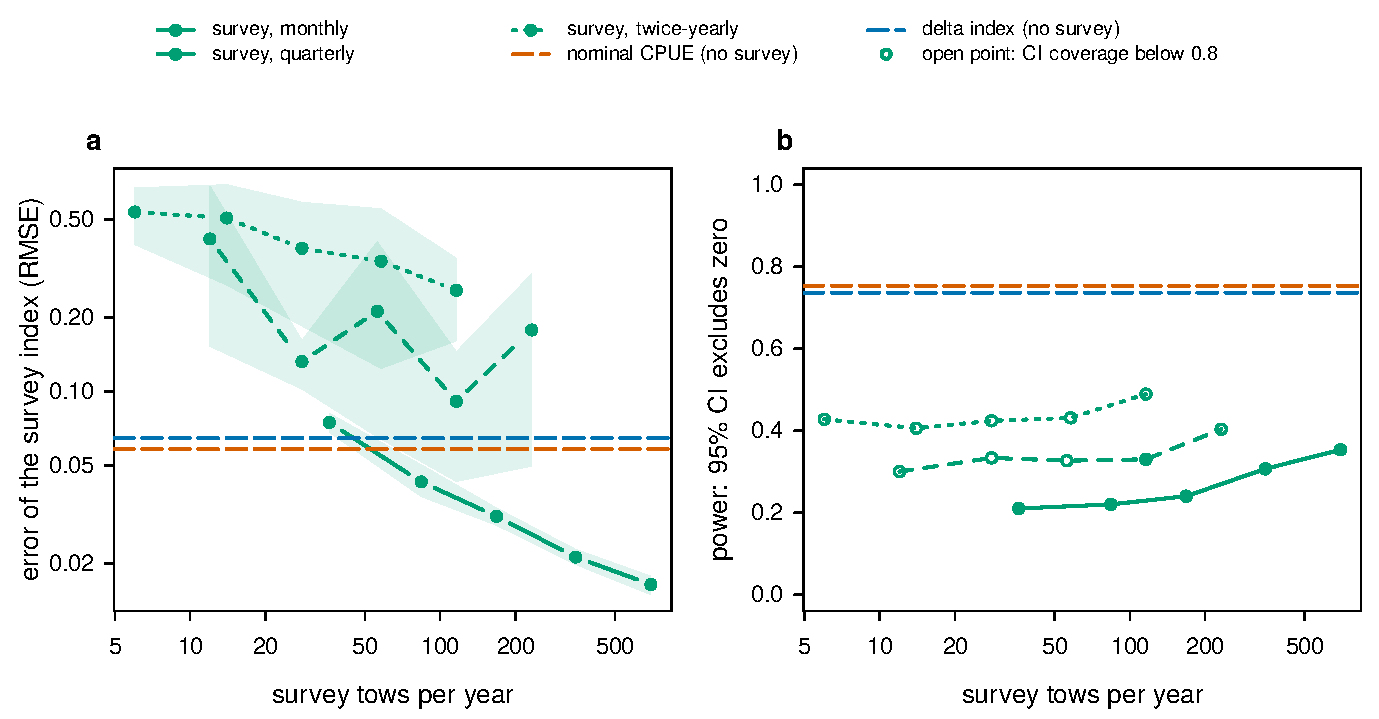
\includegraphics[width=\linewidth]{fig6_survey_coverage.pdf}
\caption{Survey design curve for the scenario with abundance decline, uniform catchability loss and fleet contraction (300 replicates per design). (a) Root mean squared error of the survey index against the true effect, by survey tows per year (both axes logarithmic), for monthly, quarterly and twice-yearly simple random surveys, with bootstrap 95 percent bands; the dashed horizontal lines are the two fishery indices, which do not use the survey. (b) Power to reject a zero effect. Open points mark designs whose 95 percent intervals contain the truth in fewer than 80 percent of replicates, for which power is not meaningful.}
\label{fig:design}
\end{figure}

\subsection{The edge of the frame sets the direction of the boundary flow}
\label{sec:res-frame}

The direction of redistribution across the frame boundary depends on conditions beyond the frame, and the survey tracks that direction (Figure~S3, Table~S5; values with fleet contraction active). When the refuge beyond the poleward edge warms with the frame, events move about 3 percent of the stock out of it, producing an in-frame effect of $-$0.010 that the survey recovers ($-$0.010). When the refuge instead keeps a fixed, near-optimal suitability, the direction reverses: a heatwave warms the cooler part of the frame toward the optimum, about 2.5 percent of the stock moves in, the in-frame effect becomes 0.007, and the survey reads 0.008. The boundary flow is set by the thermal conditions inside and outside the frame relative to the species' optimum, so a warming baseline that carries the frame past the optimum increases the outflow; the sensitivity analysis (Section~\ref{sec:res-sens}) shows the survey's bias for total abundance growing with the warming trend. The nominal index, by contrast, declines under redistribution in every frame setting ($-$0.036 closed, $-$0.045 warming refuge, $-$0.028 static refuge), so its sign is not set by the direction of flow across the boundary; a plausible explanation is that a fleet allocating effort from recent catch rates lags a moving stock and keeps fishing where catch rates are falling.

\subsection{A distributed lag describes the lagged response but does not predict better}
\label{sec:res-temporal}

A same-month model cannot represent a response that accumulates over time; the distributed lag captures that structure. Fitted to the detrended survey index, it raises the coefficient of determination from 0.02 to 0.19 and the correlation of the fitted series with the true heatwave effect from 0.09 to 0.24, and its lag weights spread across the window as the cumulative response requires (Figure~S4; Table~S6); fitted to the true effect itself, it reaches a correlation of 0.51 against 0.14. Prediction tells a different story: in blocked out-of-sample validation with smoothing re-selected in each training block, the distributed lag does not outperform the same-month model (root mean squared error 0.55 versus 0.44 on the survey index), because its flexibility adds more variance than it removes bias. It is the better description of the mechanism, not the better short-horizon predictor.

\subsection{What drives the results}
\label{sec:res-sens}

The bias of the nominal index is governed above all by the size of the uniform catchability loss (standardised regression coefficient $-$0.58), the structural confound of Section~\ref{sec:res-ident}, and by the number of events ($-$0.31); abundance sensitivity ($-$0.20), niche breadth (0.16) and the stock's movement rate ($-$0.12) follow (Figure~\ref{fig:sens}, Table~S7). The strength of the fleet's contraction has almost no effect within the range tested (0.004), and the fleet's learning rate little (0.07). The survey's error against in-frame abundance depends on its own design, through coverage ($-$0.44) and encounter scale ($-$0.36), and on the size of the effect being estimated (abundance sensitivity, 0.33). Its bias against total abundance depends on the settings that govern how much of the stock crosses the frame edge, chiefly the movement rate ($-$0.38), the number of events ($-$0.36), the warming trend ($-$0.24) and niche breadth (0.18); no fleet parameter has a coefficient larger than 0.09 in magnitude. Together the fifteen parameters explain 53 percent of the variation in the nominal bias, so these coefficients rank the influences rather than predict outcomes at a given setting.

\begin{figure}[tbp]
\centering
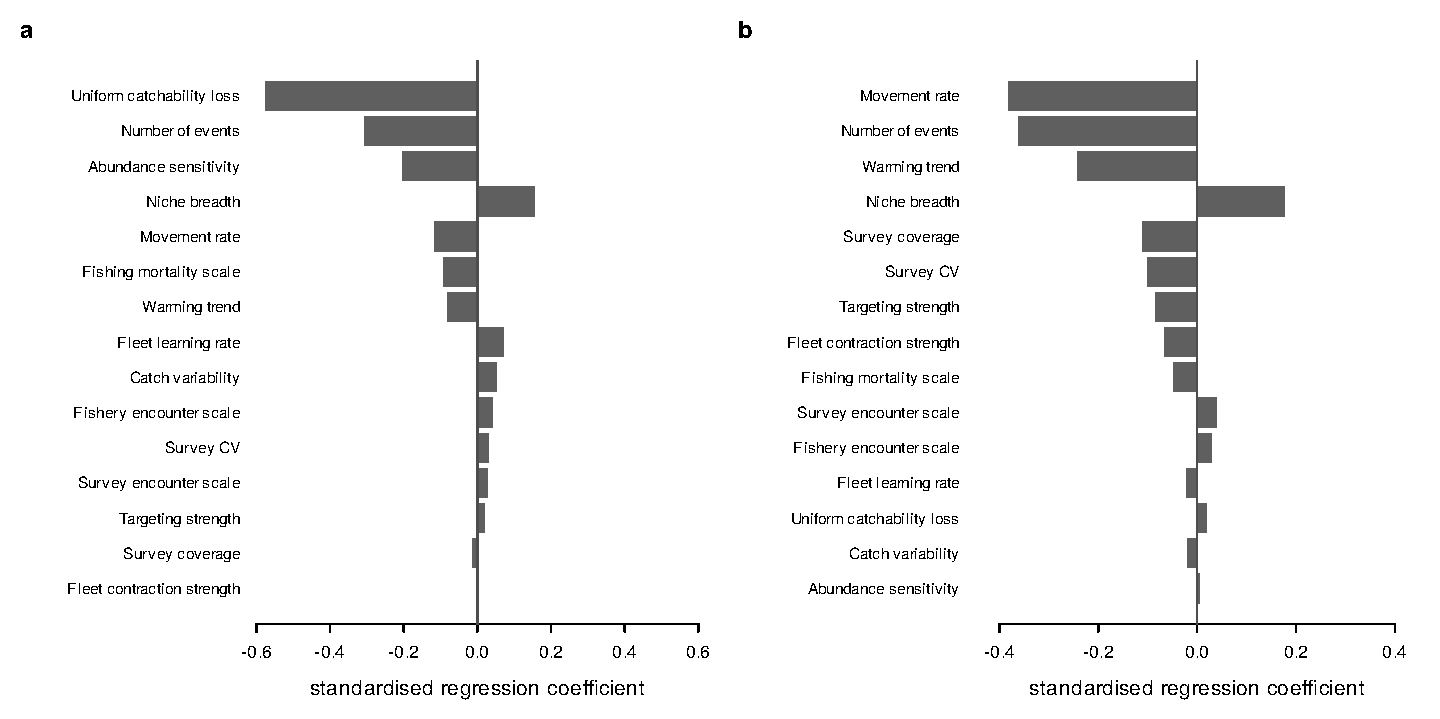
\includegraphics[width=\linewidth]{fig12_sensitivity.pdf}
\caption{Global sensitivity analysis. Standardised regression coefficients of (a) the bias of the nominal index against total abundance and (b) the bias of the survey index against total abundance, on the fifteen parameters of the design (200 design points, 20 replicates each, all mechanisms active; parameters as in Table~S1). The parameters jointly explain 53 percent of the variation in (a) and 40 percent in (b).}
\label{fig:sens}
\end{figure}

\subsection{A diagnostic key and its error rate}
\label{sec:res-key}

A simple decision key built on the joint signatures of the indices names the correct mechanism for 51 percent of test replicates across six classes, against about 17 percent by chance, and declines to classify 11 percent (Table~S8). Warm-edge catchability loss is recognised in 77 percent of its test replicates and redistribution (including warm-edge loss with redistribution) in 56 percent. Abundance decline is the most difficult class: only 25 of 194 replicates are classified correctly, and most are labelled no effect (98) or indeterminate (42), because a decline of this size is often too small for the survey to detect at the default coverage (Section~\ref{sec:res-survey}). The key's weakest point is a modest decline, which it misses far more often than it mislabels.

% =============================================================================
\section{Discussion}

\subsection{A heatwave attribution problem that fishery data alone cannot solve}

The principal result is that a decline in CPUE cannot, from fishery catch, effort and location data alone, be attributed to abundance decline or to a spatially uniform reduction in catchability. This is not a consequence of limited data, imperfect standardisation or insufficient sample size; abundance and uniform catchability occupy the same direction of the fishery likelihood, so it is an identification failure rather than a bias problem. The difficulty of detecting heatwave effects even in fishery-independent survey data \citep{fredston2023} sharpens the point: if impacts are hard to detect under a fixed sampling design, they are harder still to infer from commercial catch rates, where abundance, availability and catchability are entangled. Our power analysis reaches the same conclusion by an alternate route: the survey, which is free of catchability confounding, rejected a zero effect in only a minority of replicates at station counts that already outperformed every fishery index.

\subsection{From confounding mechanisms to monitoring solutions}

The constructive contribution of this study is the mapping from each source of confounding to the information required to resolve it (Table~\ref{tab:synthesis}). Redistribution within the observed range has a partial fishery-only remedy. When catchability is unchanged, a spatially explicit standardisation whose density surface can move with the event removes most redistribution bias, and the centre of gravity of that surface captures much of the movement. Uniform catchability change has no equivalent remedy. No covariate describing the fishing operation observes it, and the information needed to distinguish it from abundance must therefore come from outside the catch and effort records. Spatially structured catchability lies between these extremes. Fishery data can detect it, but the resulting signal imitates redistribution in the fishery centre of gravity, and only an independent survey centre of gravity distinguishes real movement from a warm-edge catchability artefact.

Availability responses during marine heatwaves are themselves diverse. Modelling of fourteen top predators across four Northeast Pacific heatwaves revealed responses ranging from near-complete habitat loss to substantial habitat expansion, varying among species and events \citep{welch2023}. Simulation studies have likewise shown that fishery-dependent sampling can recover abundance patterns under favourable spatial overlap between effort and biomass but degrades as that overlap weakens \citep{ducharme2022}, motivating specialised methods for analysing fishery-dependent distributions \citep{karp2023}. Our results are consistent with that literature and add an identifiability perspective by specifying when the limitation lies in the information content of the data rather than in the model fitted to them. Information the fishery collects beyond catch, effort and location can change that verdict. Size and age composition, tagging and controlled fishing experiments all carry information about catchability that catch rates do not, and incorporating them is the natural way to relax the invariance of eq.~\eqref{eq:invariance} without a survey.

\begin{table}[tbp]
\centering\footnotesize
\caption{What catch rates can and cannot reveal about a heatwave, and what resolves each case, in our simulation setting.}
\label{tab:synthesis}
\begin{tabular}{@{}>{\raggedright\arraybackslash}p{0.2\linewidth}>{\raggedright\arraybackslash}p{0.3\linewidth}>{\raggedright\arraybackslash}p{0.32\linewidth}l@{}}
\toprule
Mechanism & What fishery CPUE shows & What resolves it & Section \\
\midrule
Abundance decline alone & recovered by any index that keeps zero catches, provided the other mechanisms are absent & confirmation that they are absent, which needs the rows below & \ref{sec:res-factorial} \\
Uniform catchability loss & read as a decline by every fishery index & a survey with fixed protocol and design-based effort & \ref{sec:res-ident}, \ref{sec:res-factorial} \\
Redistribution within the frame & false or exaggerated decline in the nominal and delta indices & spatial delta index, partly and only if catchability is unchanged; survey index and centre of gravity & \ref{sec:res-factorial}, \ref{sec:res-cog} \\
Redistribution across the frame edge & the in-frame decline is visible; the proportion that left, and hence the total effect, is not & a survey frame that extends beyond the historical range & \ref{sec:res-factorial}, \ref{sec:res-frame} \\
Warm-edge catchability loss & fishery centre of gravity shifts, imitating redistribution & survey centre of gravity, which does not move & \ref{sec:res-cog} \\
Lagged, cumulative decline & shape missed by a same-month model & distributed lag, as a description rather than a predictor & \ref{sec:res-temporal} \\
Survey requirement & & monthly sampling; 7 to 14 stations a month outperformed every fishery index; twice-yearly sampling cannot separate event from season & \ref{sec:res-survey} \\
\bottomrule
\end{tabular}
\end{table}

\subsection{What fishery-independent surveys actually estimate}

Surveys help because effort is allocated independently of abundance and catchability is fixed and known, but what they estimate is abundance within the sampling frame, and whether that is the relevant management quantity depends on the decision context. If biomass that moves beyond the boundary is effectively unavailable to the fishery, then in-frame abundance is the appropriate target and the survey is unbiased for it. If the boundary is administrative and displaced biomass remains part of the managed stock, then total abundance becomes the target and the survey will overstate decline whenever individuals leave the frame. The frame geometry experiment shows that the magnitude, and even the direction, of this discrepancy depends on thermal conditions beyond the sampled area (Section~\ref{sec:res-frame}). Defining the target quantity is therefore a prerequisite for survey design. Where total stock abundance is the management objective, survey coverage should extend beyond the historical distribution of the stock wherever practical.

Redistribution and abundance decline also commonly occur together. Although often presented as competing explanations for declining catch rates, a global analysis of 2,572 marine fish population trends found that rapid poleward range shifts were generally associated with local population declines rather than stable abundance \citep{chaikin2024}. A falling CPUE therefore cannot safely be interpreted as a purely spatial phenomenon. If redistribution and decline are correlated, attributing a catch-rate change to one mechanism when the other is present may substantially underestimate risk.

\subsection{Relation to previous work}

The redistribution results show that the sign of CPUE bias depends on fleet behaviour. Redistribution reduced nominal CPUE in every frame configuration, including a closed frame in which biomass merely concentrated, which contrasts with the classic expectation of hyperstability \citep{harley2001,erisman2011}. The simulated fleet learns from recent catches and so lags a stock that moves on shorter time scales; consistent with this, the sensitivity analysis shows redistribution bias growing with movement speed and weakening slightly as fleet learning accelerates, whereas event-driven contraction has little influence. Hyperstability is therefore a consequence of how fleets respond to redistribution, not of redistribution itself. By the same argument as Section~\ref{sec:invariance}, an integrated index that forces fishery and survey data to share a common temporal effect would absorb fishery catchability changes into that effect, so we benchmarked the two separately.

\subsection{Implications for monitoring marine heatwaves}

For management agencies, the results translate into monitoring decisions that must be taken before the next heatwave, since a baseline cannot be reconstructed afterwards. In our setting, sampling frequency mattered more than station count: monthly surveys separated heatwave effects from seasonality and outperformed every fishery index with seven to fourteen stations per month, whereas quarterly surveys never matched the fishery indices and twice-yearly surveys failed altogether. Survey frames should extend beyond historical stock distributions whenever total abundance is the target, and protocols should stay fixed so that catchability does not vary with conditions.

Surveys cost money, and many fisheries are assessed from commercial data alone. The survey that outperformed every fishery index in our setting was small, a few stations visited monthly, and what it buys is not precision but the ability to tell a decline from a catchability change at all. The relevant comparison is with the cost of the management error that fishery data alone cannot rule out, a quota cut after a catchability change or an unchanged quota after a decline, rather than with the cost of a larger survey. Where no survey is possible, fishery data still retain an important role. Spatial standardisation removed most redistribution bias whenever catchability remained stable, and the comparison between fishery and survey centres of gravity distinguished movement from spatially varying catchability. Recording where and how fishing occurred, and not only how much was caught, is what makes those comparisons possible.

\subsection{Limitations and extensions}

The operating model is deliberately simple, a stylised grid with a single environmental driver and a thermal niche, designed to make the truth observable rather than to reproduce a specific fishery. The structural identifiability result is general because it arises from the observation model itself, but the finite-sample quantities reported here, including station counts, sampling frequencies and error rates, are orders of magnitude rather than universal thresholds. Catch does not deplete local biomass, which excludes one important route to hyperstability: the sequential depletion of aggregations that is well documented in sedentary invertebrates and aggregating finfish, and that would make the fishery signal still harder to read in those fisheries. The delta models estimate many parameters from sparse data and may be subject to incidental-parameter bias \citep{neyman1948}, which we assessed by simulation rather than theory. The Newey--West intervals undercover somewhat for monthly surveys and badly for twice-yearly ones, which we report rather than correct. The survey is idealised, with known inclusion probabilities and fixed catchability; real surveys face design and observation challenges that would raise sampling requirements. Finally, the factorial treats mechanisms as separable switches, whereas abundance change, redistribution and catchability change often arise together from the same driver. None of these alters the central conclusion, which rests on the structure of the observation process rather than on the details of the simulated system.

\subsection{Application to real fisheries}

The framework applies to any fishery in which heatwave impacts are inferred from catch rates. The 2010--11 Western Australian marine heatwave, driven by an anomalously strong Leeuwin Current during an extreme La Ni\~{n}a \citep{pearce2013,feng2013}, is a natural setting: it was followed by recruitment failures in scallop, prawn and blue swimmer crab fisheries, prompted effort reductions and closures, and the assessment of that response called for early detection of abundance change, preferably through pre-recruit surveys \citep{caputi2016,caputi2019}. Independent information of that kind is what this framework identifies as necessary, and a finfish stock such as Spanish mackerel could support an operating model informed by observed environmental conditions, fishery behaviour and survey design.

% =============================================================================
\section{Conclusion}

Catch per unit effort cannot, on its own, tell whether a marine heatwave made a stock decline, move or merely become harder to catch, and this follows from the structure of catch and effort data rather than from a shortcoming of any particular standardisation. The way out is a different method of observation, not a better model of the catch rate. A fishery-independent survey with design-allocated effort and protocol-fixed catchability restores identifiability, is unbiased for the abundance inside its frame, and separates real movement from a warm-edge catchability change through its centre of gravity. A spatially explicit standardisation of the fishery data removes most of the redistribution bias when catchability is unchanged, but none of the bias from uniform catchability change, and no index confined to the frame can see the proportion of a stock that an event moves beyond it. How much survey is needed depends on frequency more than on station count, and the survey that sufficed here was small. For an agency facing the next heatwave, the data needed to attribute its effect must be in place before the event, and the survey's frame, frequency and target are design decisions this framework can inform.

% =============================================================================
\section*{Acknowledgements}
% AUTHORS: add funding and acknowledgements.

\noindent\textit{Use of generative AI.} The authors used Claude (Anthropic) to help write and test the R simulation code, generate figures, check references against their sources, and draft and edit the text. All code was executed in R 4.3.3, every reported number was reproduced by the authors from the archived code, and every reference was checked against the original publication. The authors take full responsibility for the content.
% AUTHORS: confirm that the reproduction and reference checks described above have been completed before submission, and adjust the statement to the journal's current policy.

\section*{Conflict of interest}
The authors declare no conflict of interest.

\section*{Data availability statement}
This study uses no empirical data. All results, tables and figures are generated by simulation from the R code described in the Methods. The code, the simulated outputs underlying every reported number, and the scripts that reproduce the tables, figures and this manuscript are available on GitHub (\url{https://github.com/EAfrifa-Yamoah/Simulation-Recovery-of-Heatwave-Effect-}) and are permanently archived on Zenodo (\url{https://doi.org/10.5281/zenodo.23293721}; \citealp{awuah2026}).
% The DOI above is the Zenodo concept DOI, which resolves to the latest version; the reference
% list cites the version DOI of release 2.0.0 (10.5281/zenodo.23629610), the code used here.

\section*{Supporting Information}
Additional Supporting Information may be found online: Section S1 (why a survey is not simply another catch rate), S2 (thermal stress beyond the frame), S3 (effort adjustment of the delta index), S4 (distributed lag model), S5 (diagnostic key), Tables S1 to S9 and Figures S1 to S4.

% =============================================================================
\begin{thebibliography}{99}
\setlength{\itemsep}{2pt}

\bibitem[Afrifa-Yamoah et~al.(2026)]{afrifa2026}
Afrifa-Yamoah, E., Awuah-Mensah, Y. K., Bradshaw, S. and Mueller, U. (2026). Climate change impacts on fish-related ecosystem services: synthesis, network analysis, and strategic pathways for coordinated adaptation. \textit{Reviews in Fish Biology and Fisheries}, 36, 51.

\bibitem[Arregu\'in-S\'anchez(1996)]{arreguin1996}
Arregu\'in-S\'anchez, F. (1996). Catchability: a key parameter for fish stock assessment. \textit{Reviews in Fish Biology and Fisheries}, 6(2), 221--242.

\bibitem[Awuah-Mensah and Afrifa-Yamoah(2026)]{awuah2026}
Awuah-Mensah, Y. K. and Afrifa-Yamoah, E. (2026). Code: Declined, displaced, or just harder to catch? A simulation framework for attributing marine heatwave impacts on fished populations from catch per unit effort (Version 2.0.0) [Computer software]. \textit{Zenodo}. \url{https://doi.org/10.5281/zenodo.23629610}

\bibitem[Babcock et~al.(2019)]{babcock2019}
Babcock, R. C., Bustamante, R. H., Fulton, E. A. et al. (2019). Severe continental-scale impacts of climate change are happening now: extreme climate events impact marine habitat forming communities along 45\% of Australia's coast. \textit{Frontiers in Marine Science}, 6, 411.

\bibitem[Caputi et~al.(2016)]{caputi2016}
Caputi, N., Kangas, M., Denham, A., Feng, M., Pearce, A., Hetzel, Y. and Chandrapavan, A. (2016). Management adaptation of invertebrate fisheries to an extreme marine heat wave event at a global warming hot spot. \textit{Ecology and Evolution}, 6(11), 3583--3593.

\bibitem[Caputi et~al.(2019)]{caputi2019}
Caputi, N., Kangas, M., Chandrapavan, A., Hart, A., Feng, M., Marin, M. and de Lestang, S. (2019). Factors affecting the recovery of invertebrate stocks from the 2011 Western Australian extreme marine heatwave. \textit{Frontiers in Marine Science}, 6, 484.

\bibitem[Chaikin et~al.(2024)]{chaikin2024}
Chaikin, S., Riva, F., Marshall, K. E., Lessard, J.-P. and Belmaker, J. (2024). Marine fishes experiencing high-velocity range shifts may not be climate change winners. \textit{Nature Ecology \& Evolution}, 8(5), 936--946.

\bibitem[Cheung and Fr\"olicher(2020)]{cheung2020}
Cheung, W. W. L. and Fr\"olicher, T. L. (2020). Marine heatwaves exacerbate climate change impacts for fisheries in the northeast Pacific. \textit{Scientific Reports}, 10, 6678.

\bibitem[Craven and Wahba(1979)]{craven1979}
Craven, P. and Wahba, G. (1979). Smoothing noisy data with spline functions: estimating the correct degree of smoothing by the method of generalized cross-validation. \textit{Numerische Mathematik}, 31(4), 377--403.

\bibitem[Ducharme-Barth et~al.(2022)]{ducharme2022}
Ducharme-Barth, N. D., Gr\"uss, A., Vincent, M. T., Kiyofuji, H., Aoki, Y., Pilling, G., Hampton, J. and Thorson, J. T. (2022). Impacts of fisheries-dependent spatial sampling patterns on catch-per-unit-effort standardization: a simulation study and fishery application. \textit{Fisheries Research}, 246, 106169.

\bibitem[Erisman et~al.(2011)]{erisman2011}
Erisman, B. E., Allen, L. G., Claisse, J. T., Pondella, D. J., Miller, E. F. and Murray, J. H. (2011). The illusion of plenty: hyperstability masks collapses in two recreational fisheries that target fish spawning aggregations. \textit{Canadian Journal of Fisheries and Aquatic Sciences}, 68(10), 1705--1716.

\bibitem[Feng et~al.(2013)]{feng2013}
Feng, M., McPhaden, M. J., Xie, S.-P. and Hafner, J. (2013). La Ni\~{n}a forces unprecedented Leeuwin Current warming in 2011. \textit{Scientific Reports}, 3, 1277.

\bibitem[Fredston et~al.(2023)]{fredston2023}
Fredston, A. L., Cheung, W. W. L., Fr\"olicher, T. L. et al. (2023). Marine heatwaves are not a dominant driver of change in demersal fishes. \textit{Nature}, 621(7978), 324--329.

\bibitem[Fretwell and Lucas(1969)]{fretwell1969}
Fretwell, S. D. and Lucas, H. L. (1969). On territorial behavior and other factors influencing habitat distribution in birds. \textit{Acta Biotheoretica}, 19(1), 16--36.

\bibitem[Fr\"olicher et~al.(2018)]{frolicher2018}
Fr\"olicher, T. L., Fischer, E. M. and Gruber, N. (2018). Marine heatwaves under global warming. \textit{Nature}, 560(7718), 360--364.

\bibitem[Fuster-Alonso et~al.(2024)]{fuster2024}
Fuster-Alonso, A., Conesa, D., Pennino, M. G. et al. (2024). Spatio-temporal sampling designs and dependence: implications for abundance indices. \textit{ICES Journal of Marine Science}, 81(5), 984--995.

\bibitem[Harley et~al.(2001)]{harley2001}
Harley, S. J., Myers, R. A. and Dunn, A. (2001). Is catch-per-unit-effort proportional to abundance? \textit{Canadian Journal of Fisheries and Aquatic Sciences}, 58(9), 1760--1772.

\bibitem[Hobday et~al.(2016)]{hobday2016}
Hobday, A. J., Alexander, L. V., Perkins, S. E. et al. (2016). A hierarchical approach to defining marine heatwaves. \textit{Progress in Oceanography}, 141, 227--238.

\bibitem[Horvitz and Thompson(1952)]{horvitz1952}
Horvitz, D. G. and Thompson, D. J. (1952). A generalization of sampling without replacement from a finite universe. \textit{Journal of the American Statistical Association}, 47(260), 663--685.

\bibitem[Hoyle et~al.(2024)]{hoyle2024}
Hoyle, S. D., Campbell, R. A., Ducharme-Barth, N. D. et al. (2024). Catch per unit effort modelling for stock assessment: a summary of good practices. \textit{Fisheries Research}, 269, 106860.

\bibitem[Karp et~al.(2023)]{karp2023}
Karp, M. A., Brodie, S., Smith, J. A. et al. (2023). Projecting species distributions using fishery-dependent data. \textit{Fish and Fisheries}, 24(1), 71--92.

\bibitem[Maunder and Punt(2004)]{maunder2004}
Maunder, M. N. and Punt, A. E. (2004). Standardizing catch and effort data: a review of recent approaches. \textit{Fisheries Research}, 70(2--3), 141--159.

\bibitem[Maunder et~al.(2006)]{maunder2006}
Maunder, M. N., Sibert, J. R., Fonteneau, A., Hampton, J., Kleiber, P. and Harley, S. J. (2006). Interpreting catch per unit effort data to assess the status of individual stocks and communities. \textit{ICES Journal of Marine Science}, 63(8), 1373--1385.

\bibitem[Maunder et~al.(2020)]{maunder2020}
Maunder, M. N., Thorson, J. T., Xu, H. et al. (2020). The need for spatio-temporal modeling to determine catch-per-unit effort based indices of abundance and associated composition data for inclusion in stock assessment models. \textit{Fisheries Research}, 229, 105594.

\bibitem[Newey and West(1987)]{newey1987}
Newey, W. K. and West, K. D. (1987). A simple, positive semi-definite, heteroskedasticity and autocorrelation consistent covariance matrix. \textit{Econometrica}, 55(3), 703--708.

\bibitem[Neyman and Scott(1948)]{neyman1948}
Neyman, J. and Scott, E. L. (1948). Consistent estimates based on partially consistent observations. \textit{Econometrica}, 16(1), 1--32.

\bibitem[Oliver et~al.(2018)]{oliver2018}
Oliver, E. C. J., Donat, M. G., Burrows, M. T. et al. (2018). Longer and more frequent marine heatwaves over the past century. \textit{Nature Communications}, 9, 1324.

\bibitem[Pearce and Feng(2013)]{pearce2013}
Pearce, A. F. and Feng, M. (2013). The rise and fall of the ``marine heat wave'' off Western Australia during the summer of 2010/2011. \textit{Journal of Marine Systems}, 111--112, 139--156.

\bibitem[S\"arndal et~al.(1992)]{sarndal1992}
S\"arndal, C.-E., Swensson, B. and Wretman, J. (1992). \textit{Model Assisted Survey Sampling}. Springer.

\bibitem[Smale et~al.(2019)]{smale2019}
Smale, D. A., Wernberg, T., Oliver, E. C. J. et al. (2019). Marine heatwaves threaten global biodiversity and the provision of ecosystem services. \textit{Nature Climate Change}, 9(4), 306--312.

\bibitem[Thorson(2019)]{thorson2019}
Thorson, J. T. (2019). Guidance for decisions using the Vector Autoregressive Spatio-Temporal (VAST) package in stock, ecosystem, habitat and climate assessments. \textit{Fisheries Research}, 210, 143--161.

\bibitem[Thorson and Barnett(2017)]{thorson2017}
Thorson, J. T. and Barnett, L. A. K. (2017). Comparing estimates of abundance trends and distribution shifts using single- and multispecies models of fishes and biogenic habitat. \textit{ICES Journal of Marine Science}, 74(5), 1311--1321.

\bibitem[Thorson et~al.(2020)]{thorson2020}
Thorson, J. T., Maunder, M. N. and Punt, A. E. (2020). The development of spatio-temporal models of fishery catch-per-unit-effort data to derive indices of relative abundance. \textit{Fisheries Research}, 230, 105611.

\bibitem[Thorson et~al.(2016a)]{thorson2016a}
Thorson, J. T., Pinsky, M. L. and Ward, E. J. (2016a). Model-based inference for estimating shifts in species distribution, area occupied and centre of gravity. \textit{Methods in Ecology and Evolution}, 7(8), 990--1002.

\bibitem[Thorson et~al.(2016b)]{thorson2016b}
Thorson, J. T., Rindorf, A., Gao, J., Hanselman, D. H. and Winker, H. (2016b). Density-dependent changes in effective area occupied for sea-bottom-associated marine fishes. \textit{Proceedings of the Royal Society B: Biological Sciences}, 283(1840), 20161853.

\bibitem[Thorson et~al.(2015)]{thorson2015}
Thorson, J. T., Shelton, A. O., Ward, E. J. and Skaug, H. J. (2015). Geostatistical delta-generalized linear mixed models improve precision for estimated abundance indices for West Coast groundfishes. \textit{ICES Journal of Marine Science}, 72(5), 1297--1310.

\bibitem[Welch et~al.(2023)]{welch2023}
Welch, H., Savoca, M. S., Brodie, S. et al. (2023). Impacts of marine heatwaves on top predator distributions are variable but predictable. \textit{Nature Communications}, 14, 5188.

\bibitem[Wilberg et~al.(2010)]{wilberg2010}
Wilberg, M. J., Thorson, J. T., Linton, B. C. and Berkson, J. (2010). Incorporating time-varying catchability into population dynamic stock assessment models. \textit{Reviews in Fisheries Science}, 18(1), 7--24.

\bibitem[Wernberg et~al.(2016)]{wernberg2016}
Wernberg, T., Bennett, S., Babcock, R. C. et al. (2016). Climate-driven regime shift of a temperate marine ecosystem. \textit{Science}, 353(6295), 169--172.

\bibitem[Wernberg et~al.(2013)]{wernberg2013}
Wernberg, T., Smale, D. A., Tuya, F., Thomsen, M. S., Langlois, T. J., de Bettignies, T., Bennett, S. and Rousseaux, C. S. (2013). An extreme climatic event alters ecosystem structure in a global biodiversity hotspot. \textit{Nature Climate Change}, 3(1), 78--82.

\end{thebibliography}

\end{document}
